% SVN info for this file
\svnidlong
{$HeadURL$}
{$LastChangedDate$}
{$LastChangedRevision$}
{$LastChangedBy$}

\chapter{Varietà topologiche}
\labelChapter{varietà}

\begin{introduction}
	‘‘Non dovete mai, mai, mai fare il taglia e incolla a mano, per carità di Dio! [...] A fare il taglia e incolla si diventa scemi.''
	\begin{flushright}
		\textsc{Simone Ramello,} studente con stress post-traumatico causato da Art Attack.
	\end{flushright}
\end{introduction}
\lettrine[findent=1pt, nindent=0pt]{L}{a} Terra è piatta o sferica? Per un topologo, la risposta è: \textit{dipende} da come la si guarda. Sappiamo che vista nello spazio la Terra è una \textit{sfera}; tuttavia, se ci troviamo in una \textit{zona piana}, nei nostri dintorni appare sufficientemente piatta. In modo analogo, su un foglio i \textit{triangoli} sono quelli ben noti con somma degli angoli interni un angolo piatto, se prendiamo tre punti ben distanti sulla Terra il ‘‘triangolo'' che otteniamo ha somma maggiore! Com'è possibile?\\
Le \textbf{varietà topologiche} sono la risposta formale a ciò: una varietà topologica è uno spazio che localmente ha le stesse proprietà di uno spazio Euclideo reale. In particolare, in questa trattazione ci occuperemo principalmente di varietà topologiche di \textit{dimensione 2} e di come poterle classificarle a meno di omeomorfismi.
\section{Varietà topologiche}
\begin{definition}{}[Localmente euclideo]
	Uno spazio topologico $X$ si dice \textbf{localmente euclideo}\index{localmente euclideo} di \textbf{dimensione}\index{dimensione} $n$ se ogni punto di $X$ ammette un intorno aperto omeomorfo ad una palla aperta $B_{\epsilon}$ di $\R^n$. Per ogni punto $x\in X$ si parla di \textbf{carta}\index{carta} $\left(U,\ \phi_x\right)$, cioè la coppia dell'intorno aperto $U\in I(x)$ omeomorfo a $\R^n$ e dell'omeomorfismo $\funct{}[\phi_x]{U}{\R^n}$.
\end{definition}
\begin{remark}{n}
	Equivalentemente, $X$ è localmente euclideo se ogni punto di $X$ ammette un aperto omeomorfo a $\R^n$. Questa definizione è lecita perché ogni palla aperta in $\R^n$ è omeomorfa a $\R^n$ e la composizione di omeomorfismi è un omeomorfismo.
\end{remark}

\begin{definition}{}[Varietà topologica]
	Uno spazio topologico $X$ si dice \textbf{varietà topologica}\index{varietà topologica} di dimensione $n$ se $X$ è di Hausdorff, connesso, a base numerabile e localmente euclideo di dimensione $n$.
\end{definition}

\begin{example}{pn}~{}
	\begin{itemize}
		\item $\R^n$ è una varietà topologica di dimensione $n$.
		\item $S^n$ è una varietà topologica compatta di dimensione $n$, in quanto per la proiezione stereografica si ha che $S\setminus\{*\}\cong \R$.
		\item $\Proj^n(\R)$ è una varietà topologica compatta di dimensione $n$.
		\item Ogni aperto connesso di una varietà topologica di dimensione $n$ è una varietà topologica di dimensione $n$.
	\end{itemize}
\end{example}
\begin{remark}{n}
	La dimensione di una varietà topologica è \textit{ben definita} per l'\textit{invarianza della dimensione}.
\end{remark}
\begin{remark}{pn}~{}
	\begin{enumerate}
		\item Una varietà topologica è c.p.a.
		\item Se $X$ è una varietà topologica di dimensione $n$ e $Y$ è una varietà topologica di dimensione $m$ allora $X\times Y$ è una varietà topologica di dimensione $n+m$.
	\end{enumerate}
\end{remark}
\begin{proof}{n}~{}
	\begin{enumerate}[label=\Roman*]
		\item Consideriamo un punto $x_0\in X$ e la sua componente c.p.a.:
		\begin{equation*}
			C=\Set{y\in X | \exists \funct{}[\alpha]{I}{X},\ \alpha\left(0\right)=x_0,\ \alpha\left(1\right)=y}
		\end{equation*}
		Vogliamo dimostrare che $C$ è aperto e chiuso. Notiamo che per ogni $y\in C$, essendo $X$ localmente Euclideo, esiste un intorno aperto $U\in I(y)$ tale che $U\cong B_\epsilon$, per qualche $\epsilon>0$. Poiché $B_\epsilon$ è un aperto c.p.a. di $\R^n$, anche $U$ è c.p.a. per omeomorfismo. Ma allora, per giunzione di cammini, esiste un cammino da $x_0$, passante per $y$ e che congiunge un qualunque punto dell'intorno $U$, cioè $U\subseteq C$. Al variare di $y\in C$ trovo una collezione di carte $\left\{U_i\right\}_{i\in I}$ tale che $y\in U_i$ per qualche $i\in I$, quindi
		\begin{equation*}
			C\subseteq \bigcup_{i\in I} U_i.
		\end{equation*}
		Per le osservazioni precedenti, $U_i\subseteq C,\forall i\in I$. Segue che
		\begin{equation*}
			\bigcup_{i\in I} U_i\subseteq C,
		\end{equation*}
		quindi $C$ coincide con l'unione degli aperti $\left\{U_i\right\}_{i\in I}$ e dunque è \textit{aperto}.\\
		Consideriamo ora $y\in X\setminus C$: poiché $X$ è localmente euclideo, esiste un intorno aperto $U\in I(y)$ con $U\cong B_\epsilon\subseteq \R^n$ per qualche $\epsilon>0$. In particolare, $U\cap C=\emptyset$, in quanto se così non fosse potrei sempre trovare un cammino passante per un punto in $U\cap C$ che connette $x_0$ con gli altri punti di $U$. Ma allora $U\subseteq X\setminus C$, $X\setminus C$ è intorno di ogni suo punto, cioè è \textit{aperto} e pertanto $C$ è \textit{chiuso}. Ne consegue che $C$ è un aperto e chiuso in $X$ connesso con $C\neq \emptyset$, dato che $x_0\in C$. Allora $C=X$ e dunque $X$ è c.p.a..
		\item Sappiamo che $X\times Y$ è di Hausdorff, connesso e a base numerabile perché prodotto di spazi che lo sono. Consideriamo per ogni punto in $X$ e in $Y$ rispettivamente le carte $\left(U,\ \phi_x\right)$ e $\left(U,\ \phi_y\right)$, con $\funct{}[\phi_x]{U}{\R^n}$ e $\funct{}[\phi_y]{V}{\R^m}$. Consideriamo, per ogni $\left(x,\ y\right)$:
		\begin{equation*}
			\funct{}[\psi_{x,y}]{U\times V}{\R^n\times\R^m}[\left(x,\ y\right)][\left(\phi_x(x),\ \phi_y(y)\right)]
		\end{equation*}
	Si vede che $\psi_{x,y}$ è continua, biettiva perché le componenti lo sono e l'inversa $\psi_{x,y}^{-1}=\left(\phi_x^{-1},\ \phi_y^{-1}\right)$ è continua perché sono ovviamente continue le inverse degli omeomorfismi. Dunque, poiché vale per ogni $\left(x,\ y\right)\in X\times Y$, allora $X\times Y$ è localmente euclideo di $\dim n+m$ in quanto $\R^n\times \R^m\cong\R^{n+m}$.\qedhere
	\end{enumerate}
\end{proof}
\begin{example}{n}
	$T=S^1\times S^1$ è una varietà topologica di dimensione $2$.
\end{example}
\begin{theorem}{q}[Compatto, connesso, Hausdorff, localmente euclideo implica a base numerabile]\label{compattoconnessohausdorfflocalmenteuclideo}
Sia $X$ uno spazio topologico compatto, connesso, Hausdorff e localmente euclideo di dimensione $n$. Allora $X$ è a base numerabile, dunque $X$ è una varietà topologica di dimensione $n$.\qedhere
\end{theorem}
\subsection{Dimensione 1}
Analizziamo il caso delle varietà topologiche di dimensione $1$, per esempio $\R$ e $S^1$.
\begin{theorem}{q}[Classificazione delle varietà topologiche di dimensione $1$]
	Ogni varietà topologica di dimensione $1$ è omeomorfa a $\R$ se \emph{non} è compatta, oppure a $S^1$ se compatta.\qedhere
\end{theorem}
\begin{remark}{n}\label{retta2originivarietà}
La \textbf{retta con 2 origini} (sez. \ref{retta 2 origini}, pag. \ref{retta 2 origini}) è un quoziente non Hausdorff, dunque \textit{non} è una varietà topologica.
\end{remark}
	\subsection{Dimensione 2}
\begin{definition}{}[Superficie topologica]
	Una varietà topologica di dimensione $2$ si dice \textbf{superficie topologica}\index{superficie topologica}.
\end{definition}
\begin{example}{pn}~~{}
	\begin{itemize}
		\item Il \textit{piano} $\R^2$ oppure $\R^2\setminus \{n\text{ punti}\}$ sono superfici topologiche di dimensione $2$ \textit{non} compatte.
		\item La \textbf{sfera} $S^2$ è una superficie topologica compatta.
		\item Il \textbf{toro} $T=S^1\times S^1$ è una superficie topologica compatta.
		\item Il \textbf{piano proiettivo} $P=\Proj^2(\R)$ una superficie topologica compatta.
	\end{itemize}
\end{example}
Vogliamo dare una classificazione delle superfici topologiche \textit{compatte}. Innanzitutto, esaminiamo alcuni esempi di superfici compatte studiandole sul \textit{modello piano}, di cui daremo successivamente una definizione formale.
\begin{example}{pn}[Modelli piani]~{}
		\begin{itemize}
		\item Siccome $\Proj^2(\R)$ è un quoziente del disco, allora, a meno di omeomorfismo, lo si può anche vedere come un quoziente di $I\times I$ con una relazione di equivalenza sul bordo con \textit{parola} $abab$.
		\begin{center}
		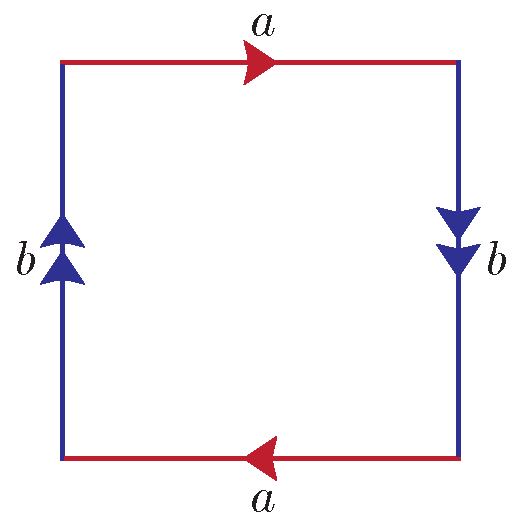
\includegraphics[trim=0cm 0cm 0cm 0cm, clip, scale=0.375]{images/proj.pdf}
		\end{center}
		\item Anche il \textbf{toro} si può vedere come quoziente di $I\times I$ con \textit{parola} $aba^{-1}b^{-1}$.
		\begin{center}
			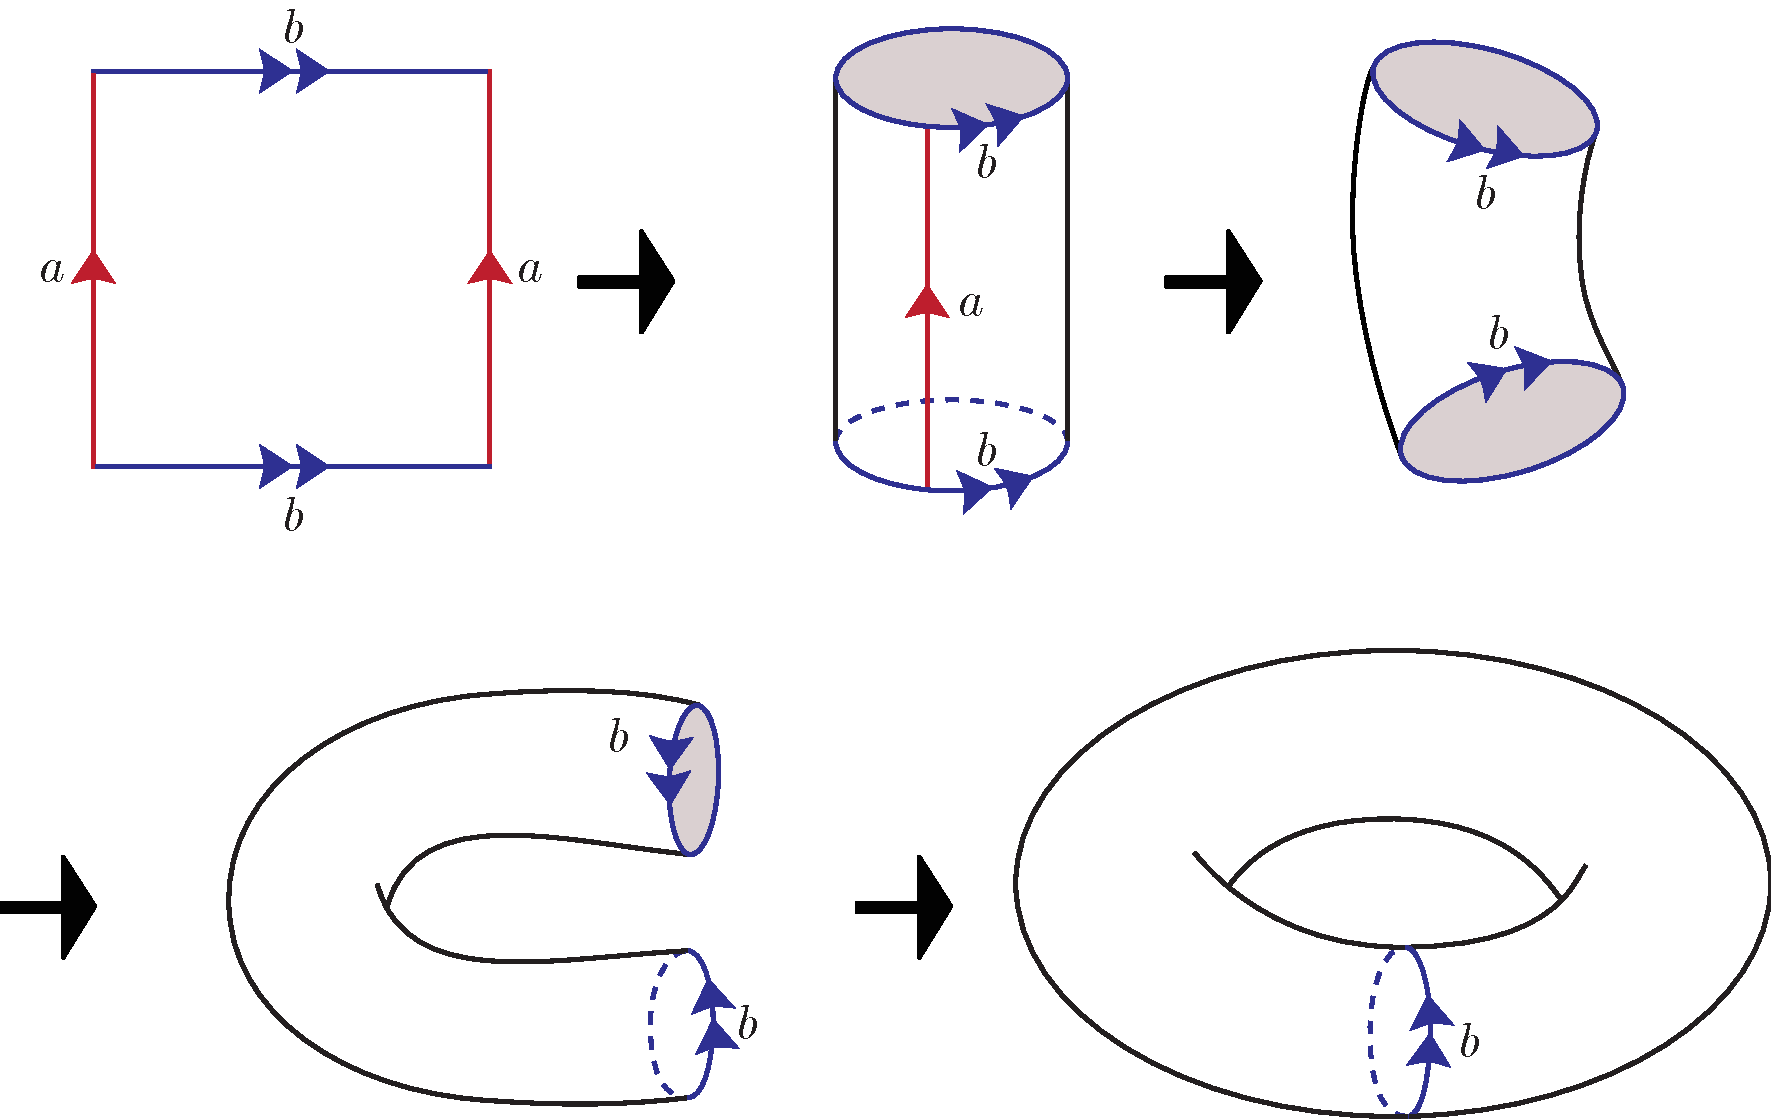
\includegraphics[trim=0cm 0cm 0cm 0cm, clip, scale=0.375]{images/torus.pdf}
		\end{center}
		\item Vediamo $S^2$ come quoziente di $I\times I$ con \textit{parola} $bb^{-1}a^{-1}a$.
		\begin{center}
			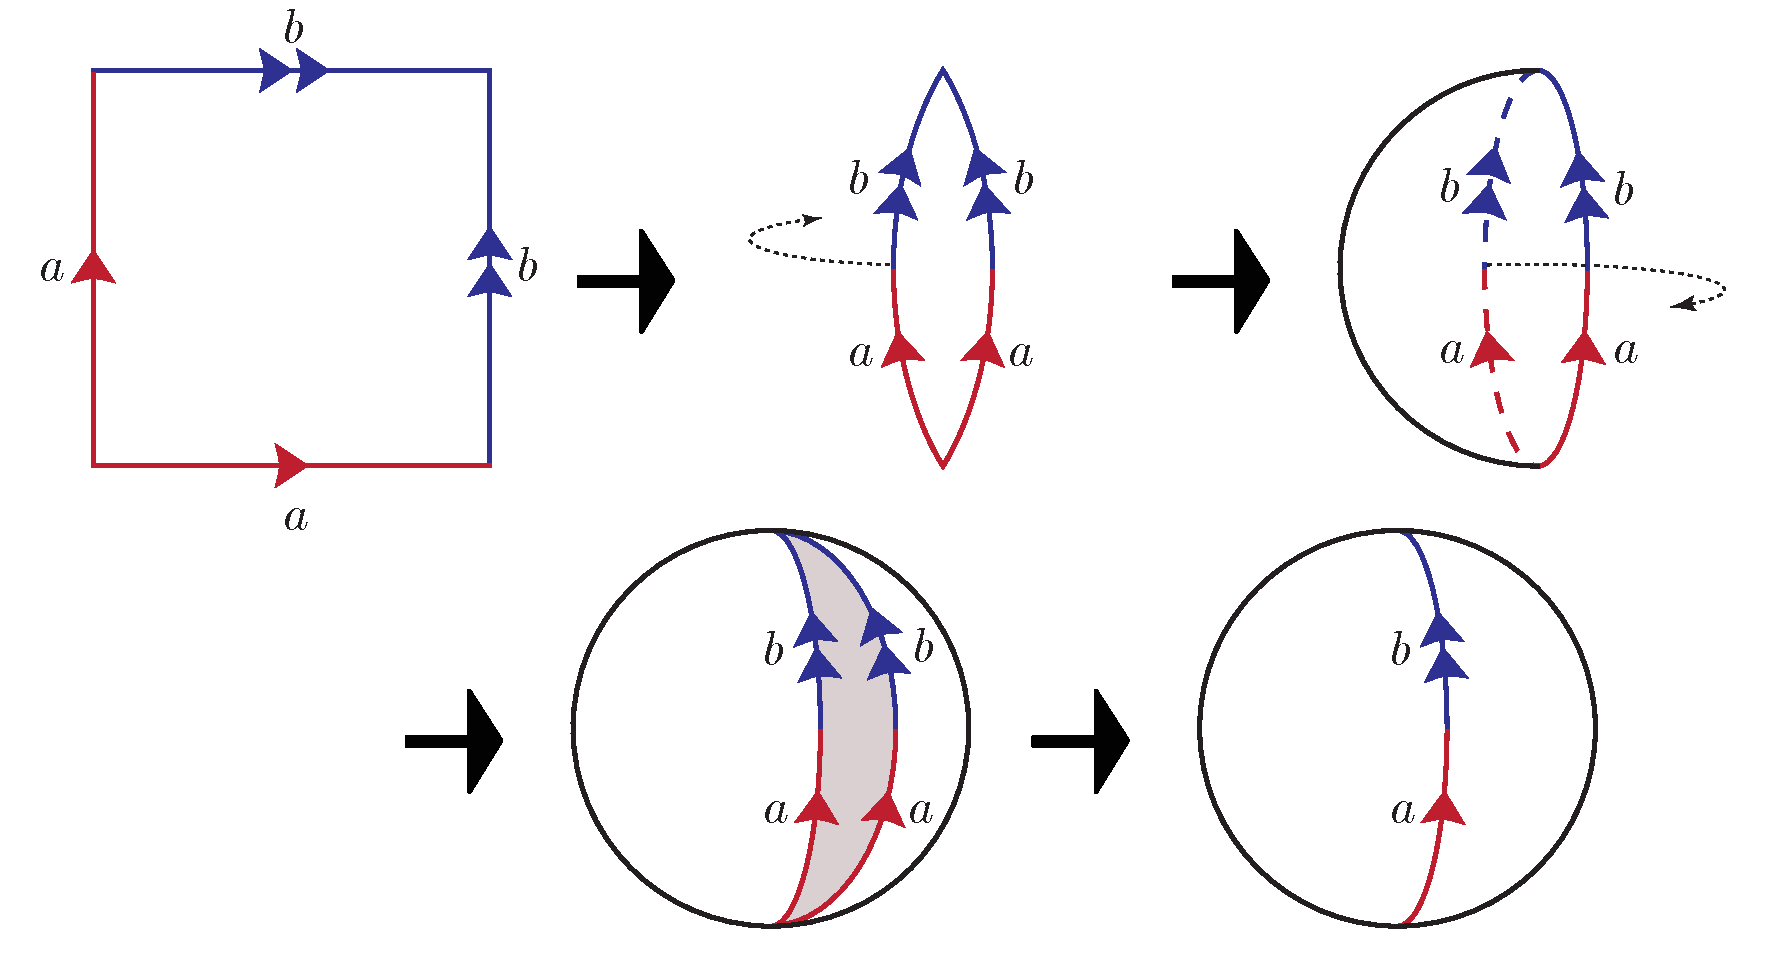
\includegraphics[trim=0cm 0cm 0cm 0cm, clip, scale=0.375]{images/sphere.pdf}
		\end{center}
	\end{itemize}
\end{example}
\begin{remark}{n}
	Sia $P\subset\R^2$ un \textit{poligono} pieno con un numero \textit{pari} di lati. Sia $\sim$ una relazione di equivalenza che identifica i lati a $2$ a $2$. Allora $S\coloneqq P/\sim$ è una \textit{superficie topologica compatta}, infatti:
		\begin{enumerate}
			\item $P$ è connesso e compatto implica che $S$ è connesso e compatto.
			\item $S$ è localmente euclideo di dimensione $2$. Infatti, sia $p\in S$:
			\begin{itemize}
				\item se $p$ viene da un \textit{punto interno} al poligono, si sceglie un intorno aperto $U$ centrato in tale punto tale che $U\cap\partial{P}=\emptyset$, in modo che $\pi(U)\cong U$ sia intorno aperto di $p$;
				\item se $p$ viene da un punto interno ad un \textit{lato}, grazie all'identificazione dei lati a due a due si ha che passando al quoziente, cioè un intorno aperto di $p$ omeomorfo ad un disco aperto;
				\item se $p$ viene da un \textit{vertice}, siccome i vertici vengono identificati con i vertici, analogamente al caso dei lati si ottiene un intorno aperto di $p$ in $S$ omeomorfo ad un disco aperto di $\R^2$.
			\end{itemize}
			\item $S$ è di Hausdorff.
		\end{enumerate}
	Poiché $l_i\cong\unint$, nella relazione di equivalenza, due lati vengono identificati scegliendo un omeomorfismo $\funct{}[\phi]{l_1}{l_2}$, in modo che $p_1\in l_1 \sim \phi(p)\in l_2$ e $\phi$ manda vertici in vertici.	Il poligono $P$ con la relazione di equivalenza sui lati è detto un \textbf{modello piano}\index{modello piano} della superficie $S$ e può essere schematizzato con una \textit{sequenza di lettere} detta \textbf{parola}\index{parola}. Ad esempio, per la parola $aba^{-1}cbc^{-1}$ si ottiene il modello piano seguente:
		\begin{center}
	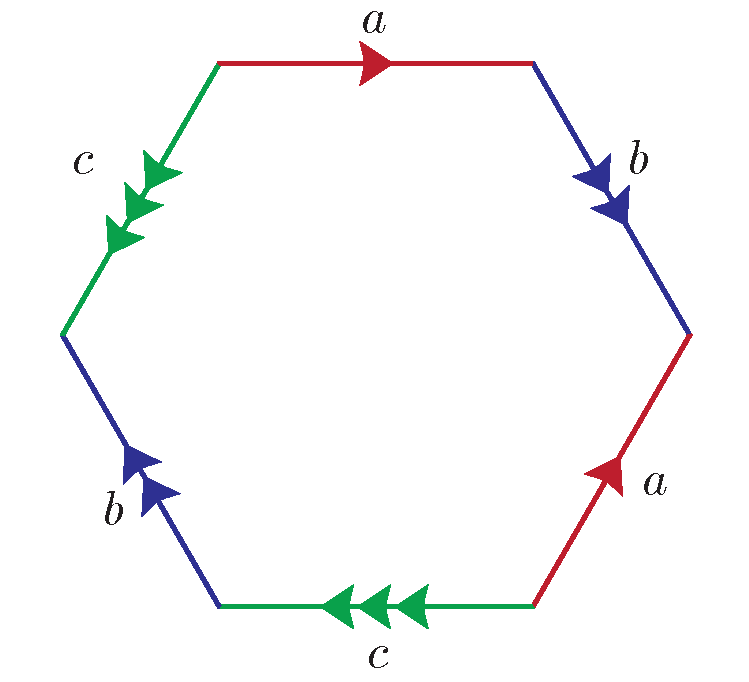
\includegraphics[trim=0cm 0cm 0cm 0cm, clip, scale=0.375]{images/modellopiano.pdf}
\end{center}
Si noti che il modello piano di una superficie compatta \textit{non è unico}.
\end{remark}
\begin{example}{pn}~{}
	\begin{itemize}
		\item Abbiamo già visto il modello piano di $S^2$ sul \textit{quadrato}; per la costruzione effettuata, possiamo unire la sequenza di lati $ab$ in un unico lato $c$ in modo da ottenere un modello costituito da un poligono \textit{improprio a due lati}, con parola $cc^{-1}$:
		\begin{center}
			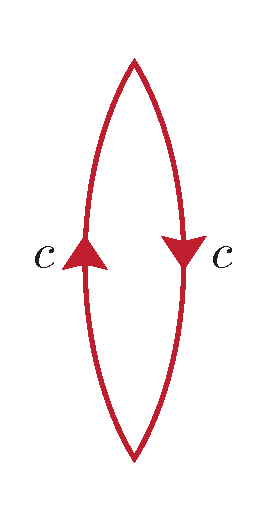
\includegraphics[trim=0cm 0cm 0cm 0cm, clip, scale=0.375]{images/sphere2lines.pdf}
		\end{center}
		\item Anche il modello piano di $\Proj^2(\R)$ sul \textit{quadrato} può essere trasformato in uno sul poligono a due lati, unificando $ba$ per ottenere un unico lato $c$ e un modello con parola $cc$:
		\begin{center}
			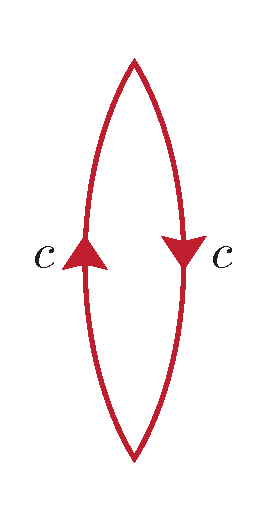
\includegraphics[trim=0cm 0cm 0cm 0cm, clip, scale=0.375]{images/proj2lines.pdf}
		\end{center}
		\item La \textbf{bottiglia di Klein}\index{bottiglia di Klein} $K$ è la superficie compatta data dal modello piano:
				\begin{center}
			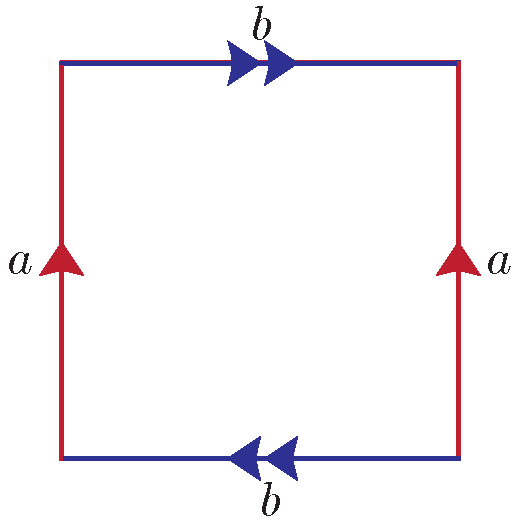
\includegraphics[trim=0cm 0cm 0cm 0cm, clip, scale=0.375]{images/klein.pdf}
		\end{center}
		Confrontiamo la costruzione della bottiglia di Klein con la costruzione del \textit{toro}, vista precedentemente. Innanzitutto otteniamo in entrambi il cilindro $S^1\times I$ con la relazione di equivalenza sul \textit{bordo}; notiamo che nella bottiglia di Klein (il modello inferiore nella figura sotto) il ‘‘verso'' rispetto al quale \textit{incolleremo} i bordi è uno l'opposto dell'altro.
		\begin{center}
			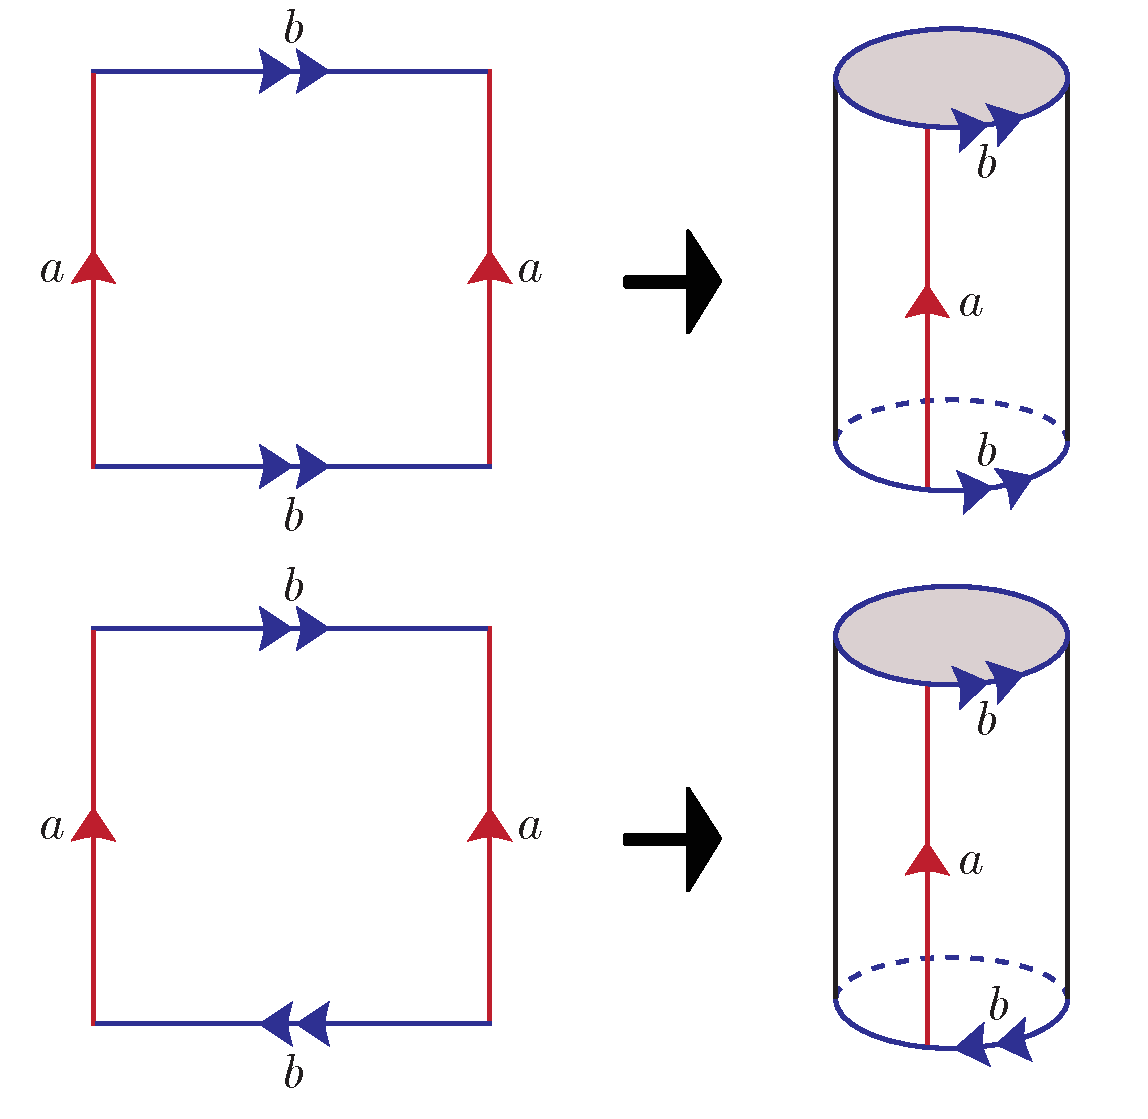
\includegraphics[trim=0cm 0cm 0cm 0cm, clip, scale=0.375]{images/kleintorus.pdf}
		\end{center}
	Questo comporta che la bottiglia di Klein \textit{non} può essere rappresentata in $\R^3$; tuttavia, possiamo visualizzarla in modo improprio operando un ‘‘\textit{taglio}'' nella superficie e compenetrando uno dei due estremi del cilindro nella figura, come di seguito.
	 \begin{center}
	 	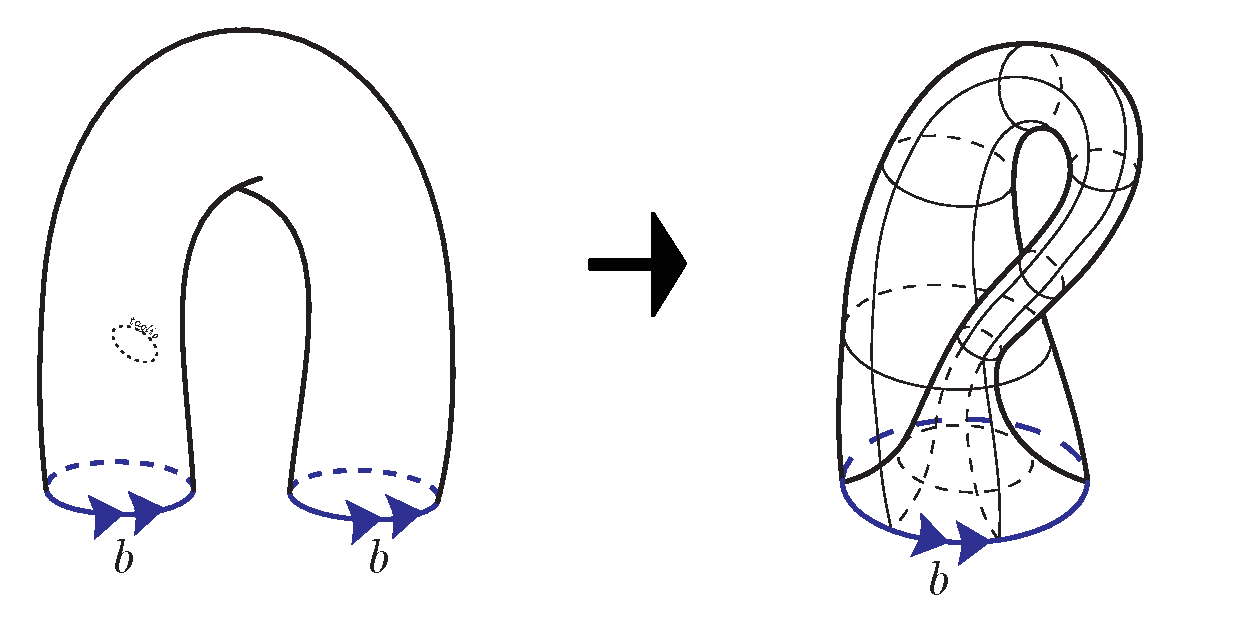
\includegraphics[trim=0cm 0cm 0cm 0cm, clip, scale=0.375]{images/kleinconstruction.pdf}
	 \end{center}
	\end{itemize}
\end{example}

\section{Somma connessa di superfici compatte}
Siano $S_1$ e $S_2$ superfici compatte e siano $x\in S_1$ e $y\in S_2$. Siano $D_x\subset S_1$ e $D_y\subset S_2$ intorni di $x$ e $y$ rispettivamente, omeomorfi entrambi ad un disco chiuso $D\subset\R^2$ tramite $h$:
% https://q.uiver.app/#q=WzAsMyxbMSwwLCJoXFxjb2xvbiBEX3giXSxbMiwwLCJEX3kiXSxbMCwwXSxbMCwxLCJcXHNpbSJdXQ==
\[\begin{tikzcd}
	{} & {h\colon D_x} & {D_y}
	\arrow["\sim", from=1-2, to=1-3]
\end{tikzcd}\]
\begin{center}
	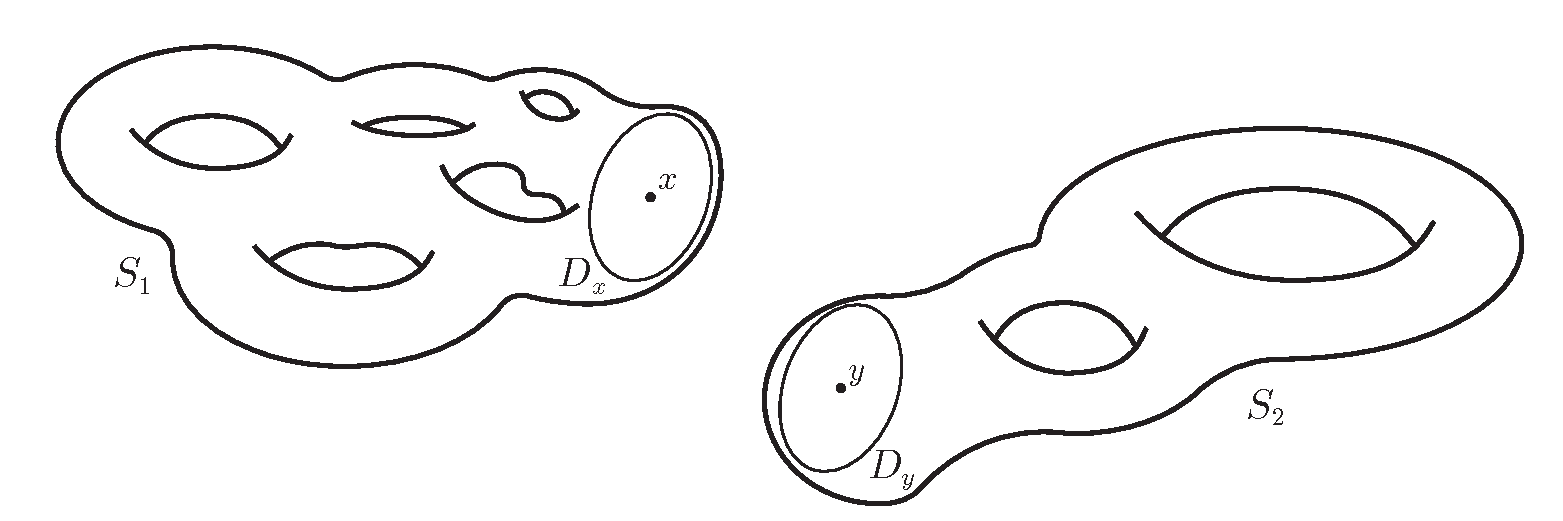
\includegraphics[trim=0cm 0cm 0cm 0cm, clip, scale=0.4]{images/connectedsum1.pdf}
\end{center}
\textit{Togliamo} dalle due superfici gli interni dei dischetti, creando dunque lo spazio
\begin{equation*}
	Y\coloneqq (S_1\setminus \interior{D_x})\amalg (S_2\setminus \interior{D_y}).
\end{equation*}
\begin{center}
	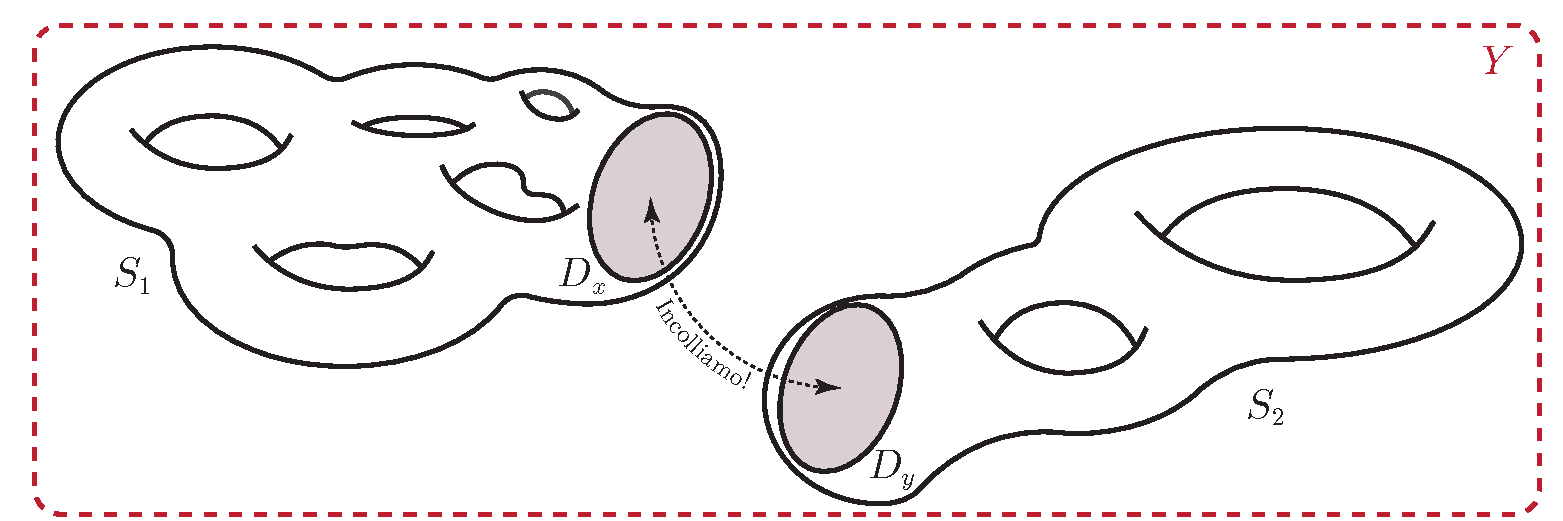
\includegraphics[trim=0cm 0cm 0cm 0cm, clip, scale=0.4]{images/connectedsum2.pdf}
\end{center}
\textit{Incolliamo} ora i due pezzi di $Y$ lungo i bordi dei dischi, cioè mettiamo su $Y$ la seguente relazione di equivalenza:
\begin{equation*}
	x_1\sim y_1 \iff x_1=y_1\text{ oppure } x_1\in\partial{D},\ y_1\in\partial{D}\text{ e } y_1=h(x_1),\ \text{o viceversa}
\end{equation*}
\begin{center}
	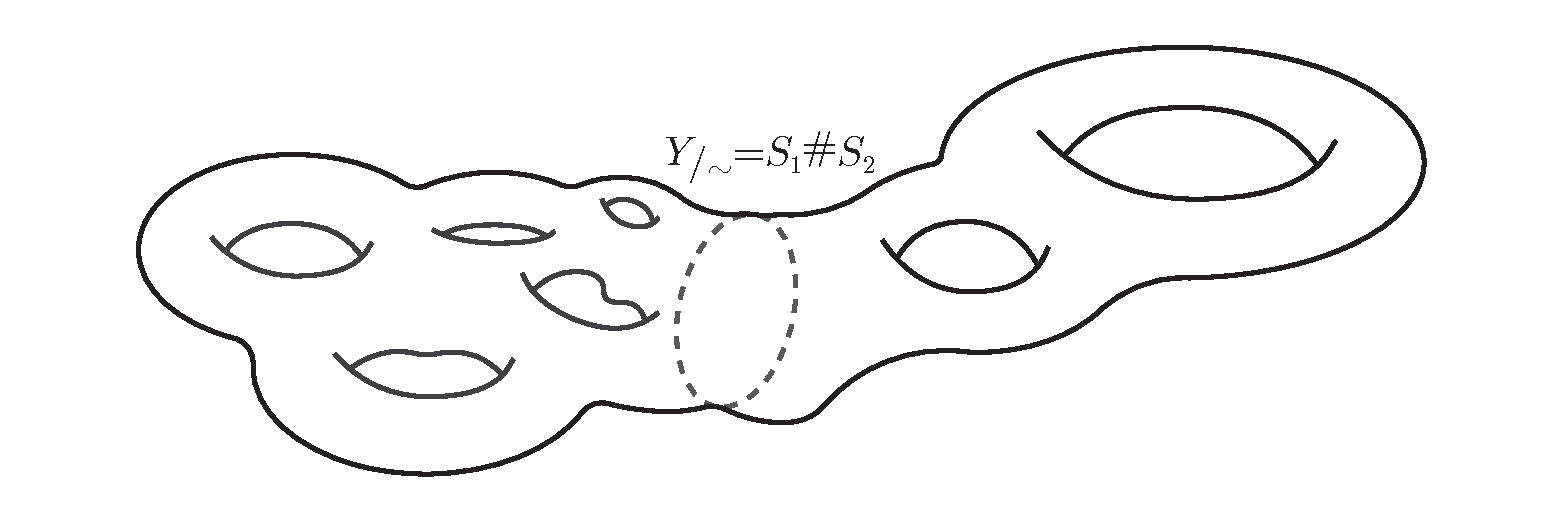
\includegraphics[trim=0cm 0cm 0cm 0cm, clip, scale=0.4]{images/connectedsum3.pdf}
\end{center}
Enunciamo ora qualche fatto che \textit{non} dimostriamo:
	\begin{itemize}
		\item il quoziente è ancora una superficie topologica, che chiamiamo \textbf{somma connessa}\index{somma!connessa} $S_1\# S_2$  di $S_1$ e $S_2$;
		\item la somma connessa $S_1\# S_2$, a meno di omeomorfismo, \textit{non dipende} dalle scelte fatte (i punti $x$ e $y$, gli intorni $D_x$ e $D_y$, l'omeomorfismo $h$) ma soltanto da $S_1$ e da $S_2$;
		\item la somma connessa di superfici compatte è, a meno di omeomorfismi, \textit{commutativa} e \textit{associativa}:
		\begin{itemize}
			\item \textbf{Commutativa}: $S_1\# S_2\cong S_2\# S_1$.
			\item \textbf{Associativa}: $\left(S_1\# S_2\right)\# S_3\cong S_1\#\left(S_2\# S_3\right)$.
		\end{itemize}
	\item se $S_1,\ S_2$ sono superfici compatte, allora $S_1\# S_2$ è una superficie compatta.
	\end{itemize}
\begin{remark}{n}
	Sia $X$ una superficie compatta. Allora $X\# S^2\cong X$. Infatti, $S^2\setminus \interior{D_y}$ è omeomorfo ad un \textit{disco chiuso} in $\R^2$. Dato che stiamo togliendo un disco anche ad $X$ per poi aggiungerne un altro, ritroviamo $X$ a meno di omeomorfismi.
	\begin{center}
		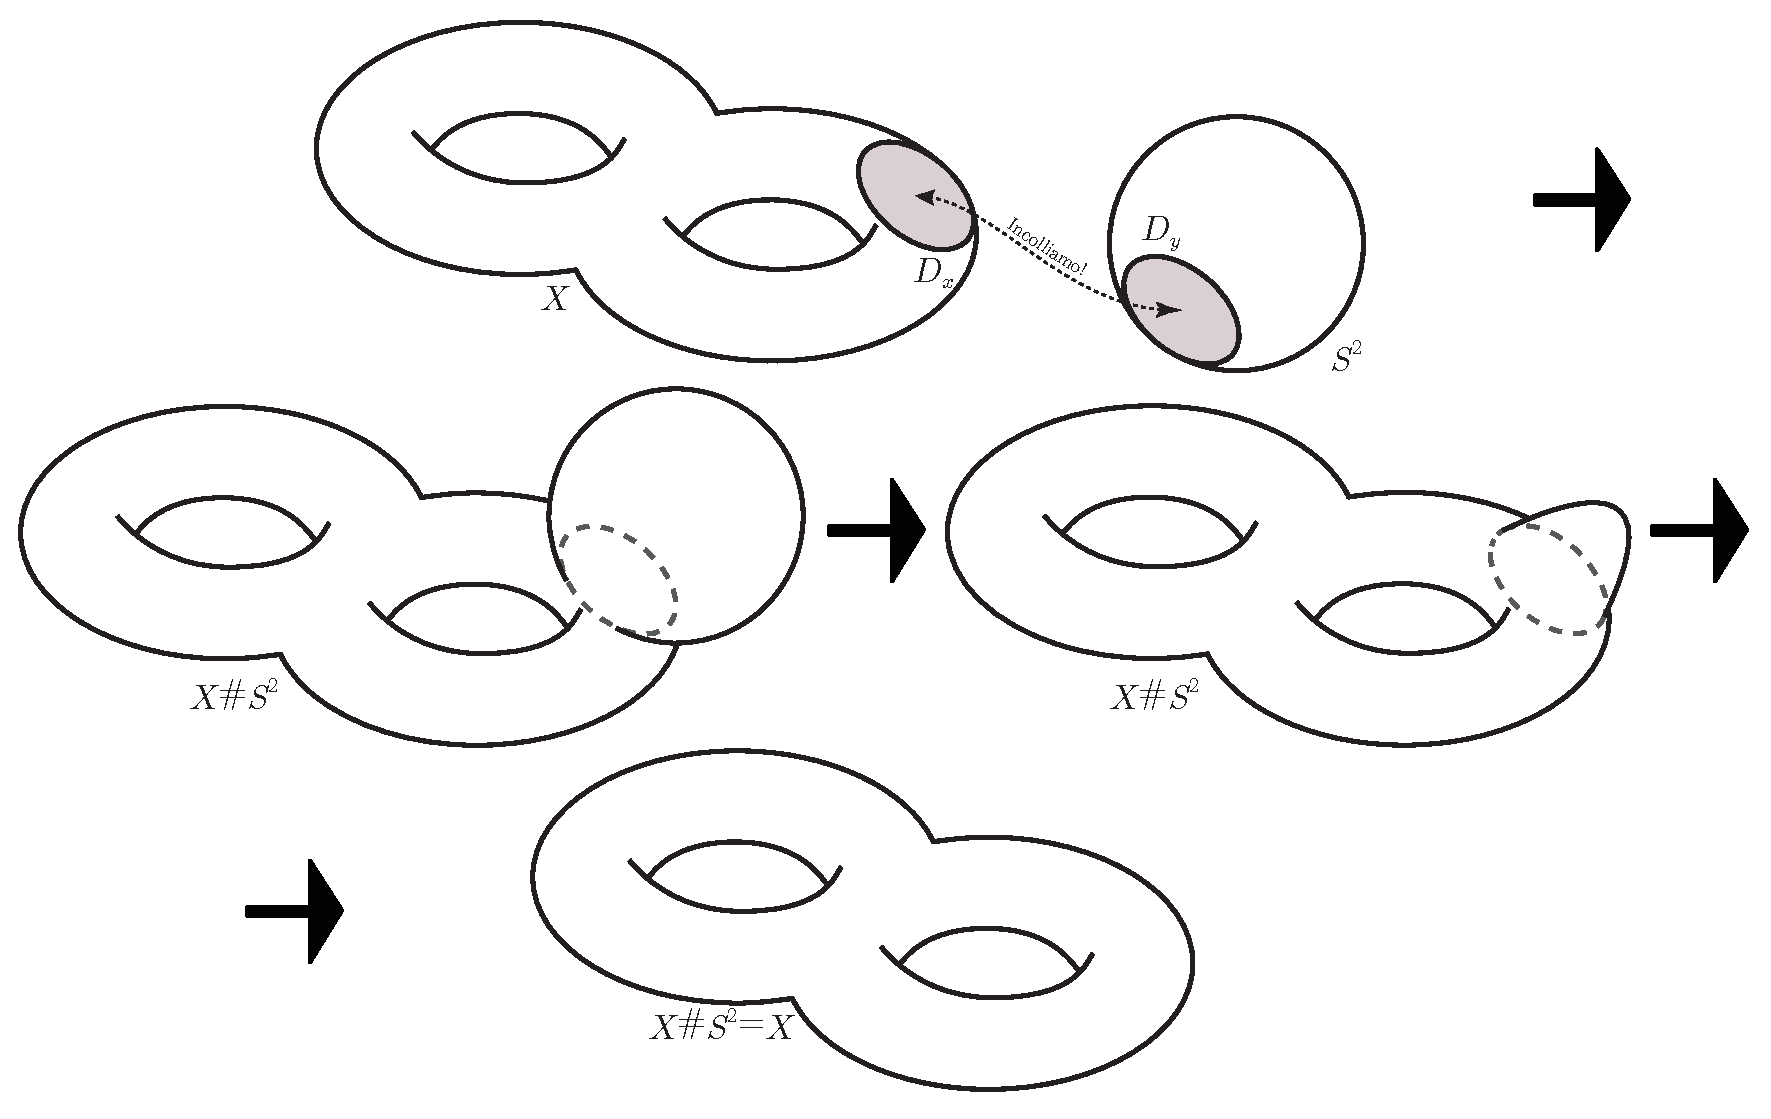
\includegraphics[trim=0cm 0cm 0cm 0cm, clip, scale=0.4]{images/connectedsumsphere.pdf}
	\end{center}
\end{remark}
\begin{definition}{}[Somma di tori]
	Indichiamo con $T_g$ la \textbf{somma connessa di }$g\geq 1$ \textbf{tori}:
	\begin{equation*}
		T_g=\underbrace{T\# \ldots\# T}_{g\ \text{volte}}\quad g\geq 1\ \left(T_1=T\right)
	\end{equation*}
$T_g$ può essere visualizzato sia come ‘‘ciambella con $g$ buchi'', sia come "sfera con $g$ manici''.
\begin{center}
	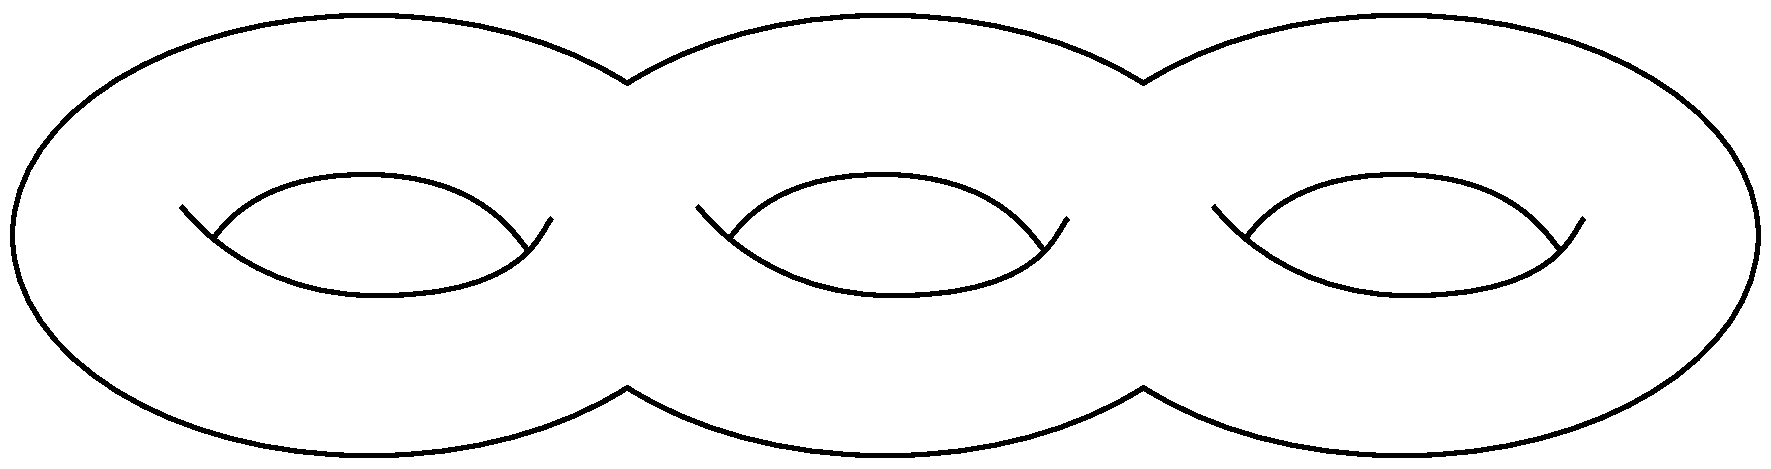
\includegraphics[trim=0cm 0cm 0cm 0cm, clip, scale=0.23]{images/toruschain.pdf}
	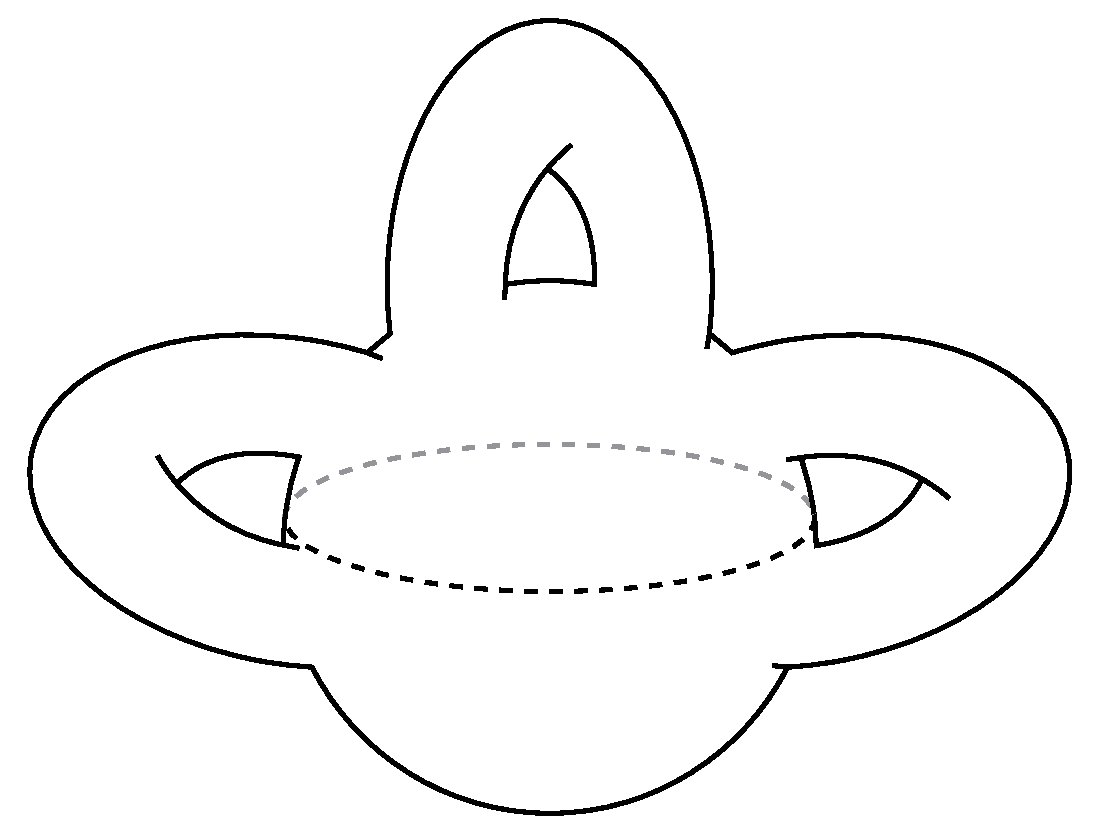
\includegraphics[trim=0cm 0cm 0cm 0cm, clip, scale=0.23]{images/spherewithhandle.pdf}
\end{center}
\end{definition}
\subsubsection{Rappresentazione della somma connessa tramite modelli piani}
\begin{minipage}{.74\linewidth}
Supponiamo che $S_1$ e $S_2$ abbiano entrambe un modello piano, rappresentato da una parola. Ad esempio, prendiamo come $S_1$ un \textit{toro}, con parola $a_1b_1a_1^{-1}b_1^{-1}$. Scegliamone un \textit{vertice} e prendiamo un disco $\overline{U}$ passante per il vertice che non tocca il resto del bordo.
\end{minipage}
\begin{minipage}{.25\linewidth}
\begin{center}
	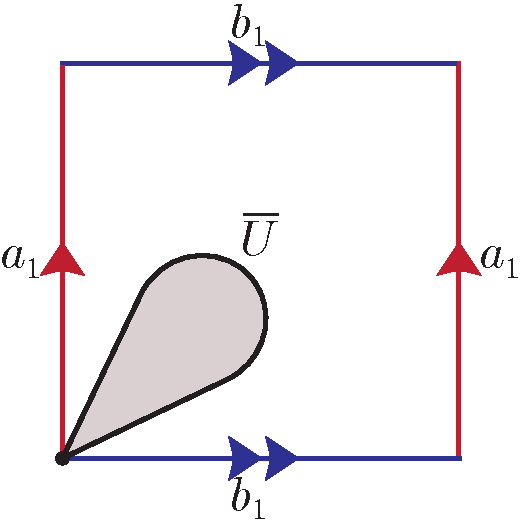
\includegraphics[trim=0cm 0cm 0cm 0cm, clip, scale=0.4]{images/torusmodelconnect1.pdf}
\end{center}
\end{minipage}~{}\\
Per fare la somma connessa, togliamo $U$:
\begin{center}
	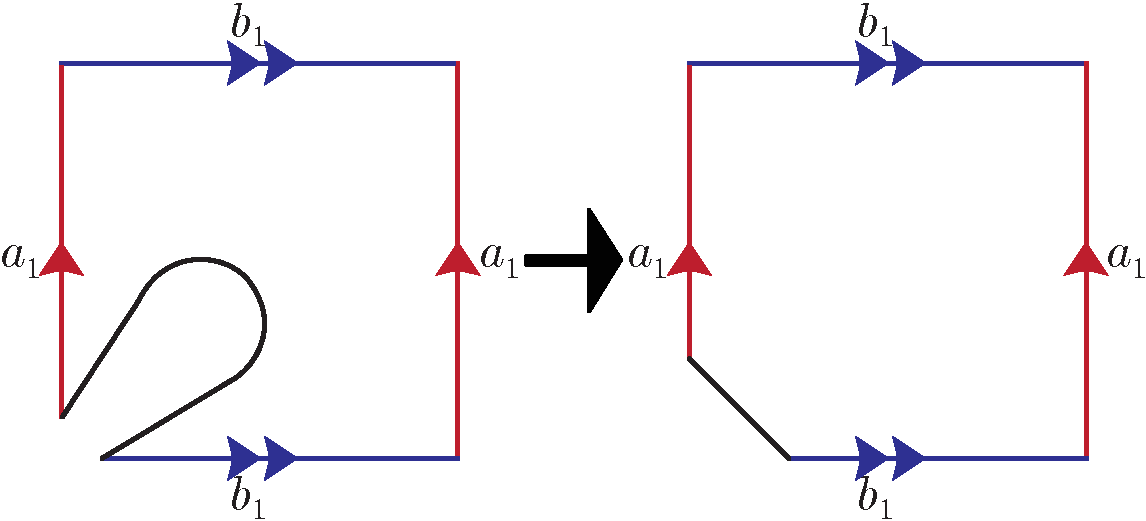
\includegraphics[trim=0cm 0cm 0cm 0cm, clip, scale=0.35]{images/torusmodelconnect2.pdf}
\end{center}
Facciamo lo stesso con la seconda superficie, $S_2$, che in questo esempio è anch'essa un toro di parola $a_2b_2a_2^{-1}b_2^{-1}$:
\begin{center}
	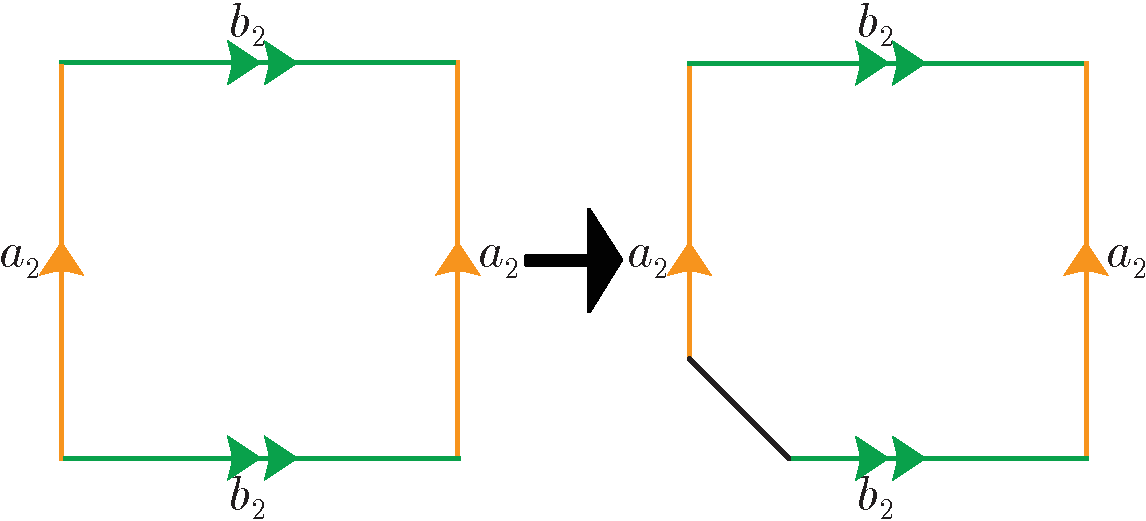
\includegraphics[trim=0cm 0cm 0cm 0cm, clip, scale=0.35]{images/torusmodelconnect3.pdf}
\end{center}
Infine, \textit{incolliamo} lungo i due nuovi lati creati bucando le due superfici:
 \begin{center}
 	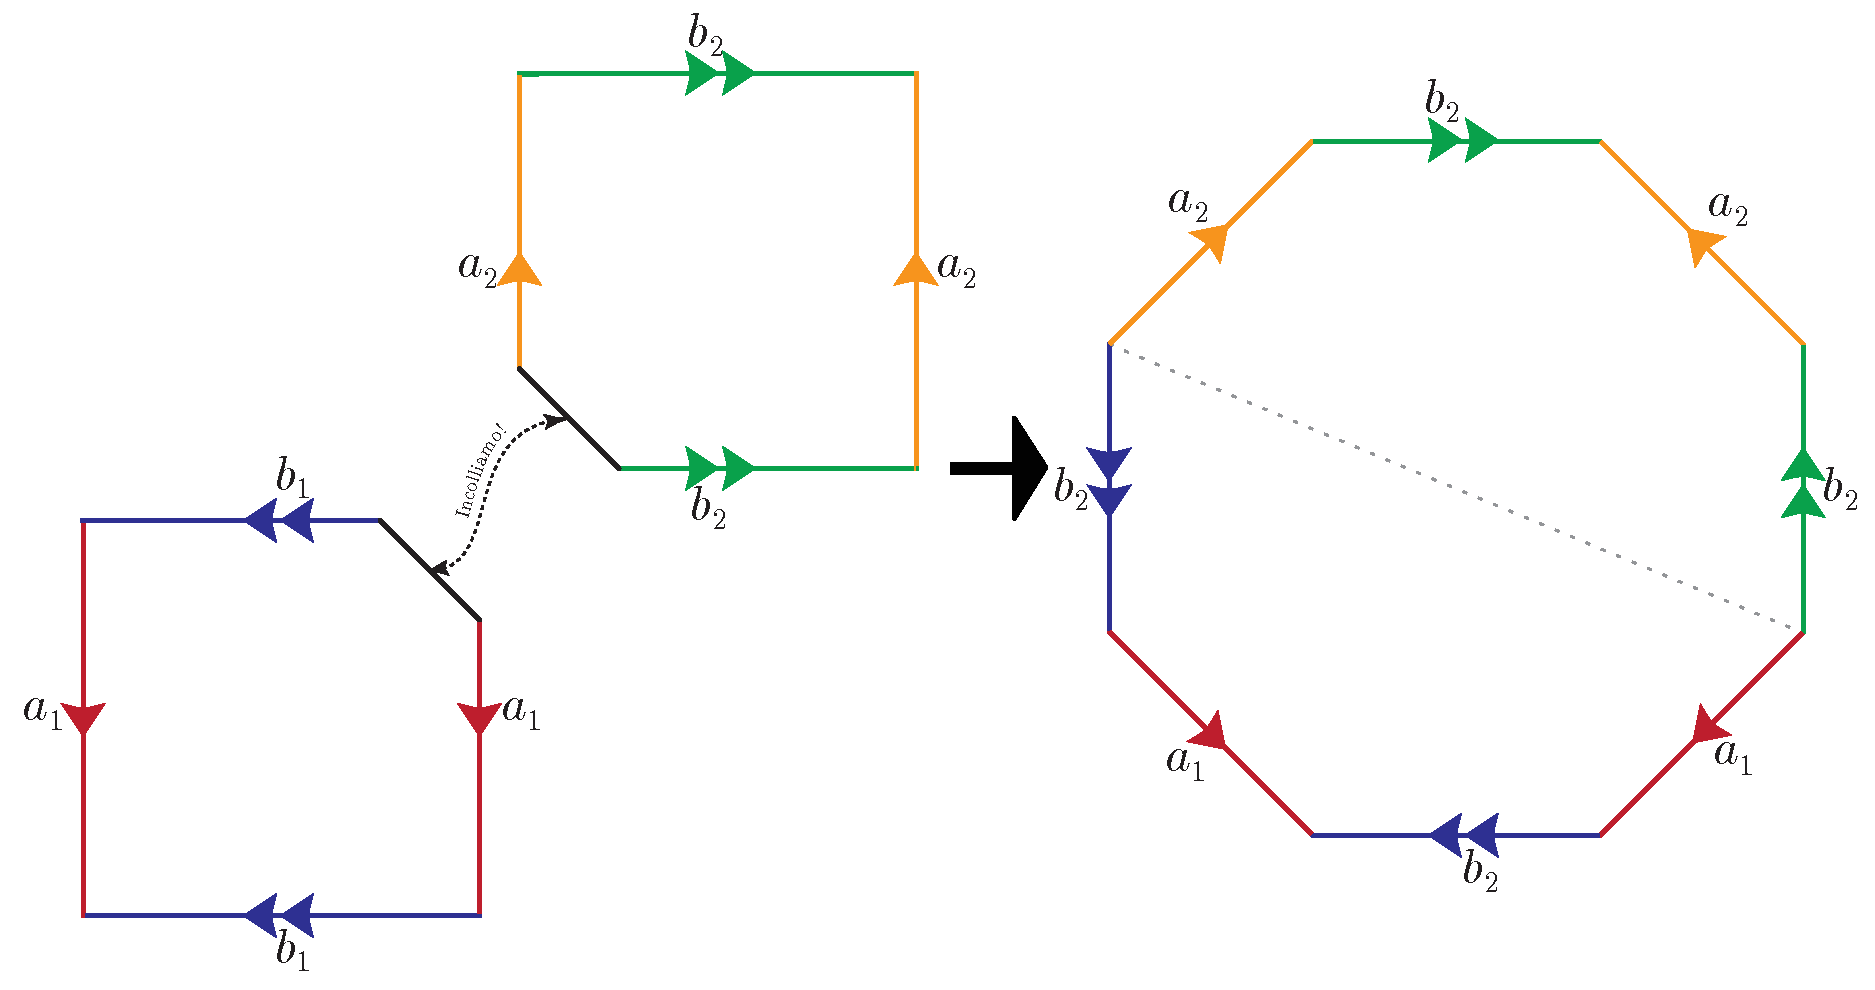
\includegraphics[trim=0cm 0cm 0cm 0cm, clip, scale=0.35]{images/torusmodelconnect4.pdf}
 \end{center}
Il modello ottenuto è un modello piano per $S_1\# S_2$, la cui parola associata è ottenuta per \textit{concatenazione}:
\begin{equation*}
	\underbrace{a_1b_1a_1^{-1}b_1^{-1}}_{\text{modello piano di }S_1}\underbrace{a_2b_2a_2^{-1}b_2^{-1}}_{\text{modello piano di }S_2}
\end{equation*}
\begin{example}{n}
Il toro $T$ è dato dalla parola $aba^{-1}b^{-1}$. Allora $T_g=T\#\ldots\# T$ è un quoziente con $4g$ lati e ha un modello piano dato dalla parola:
\begin{equation*}
a_1b_1a_1^{-1}b_1^{-1}a_2b_2a_2^{-1}b_2^{-1}\ldots a_gb_ga_g^{-1}b_g^{-1}
\end{equation*}
\end{example}
\begin{definition}{}[Somma connessa di $n$ piani proiettivi]
	Preso il \textit{piano proiettivo reale} $P=\Proj^2\left(\R\right)$, definiamo la \textbf{somma connessa di} $n$ \textbf{piani proiettivi} come:
	\begin{equation*}
		P_n=\underbrace{P\# \ldots\# P}_{n\ \text{volte}}\quad n\geq 1\ \left(P_1=P\right)
	\end{equation*}
\end{definition}
\begin{remark}{n}
	Mostriamo che la \textit{bottiglia di Klein} altro non è che la somma connessa di due piani proiettivi, cioè $K=P\# P=P_2$.\\
	\begin{minipage}{.75\linewidth}
		$K$ ha il modello piano quadrato con parola $aba^{-1}b$, come nella figura a fianco.
	\end{minipage}
	\begin{minipage}{.24\linewidth}
		\begin{center}
			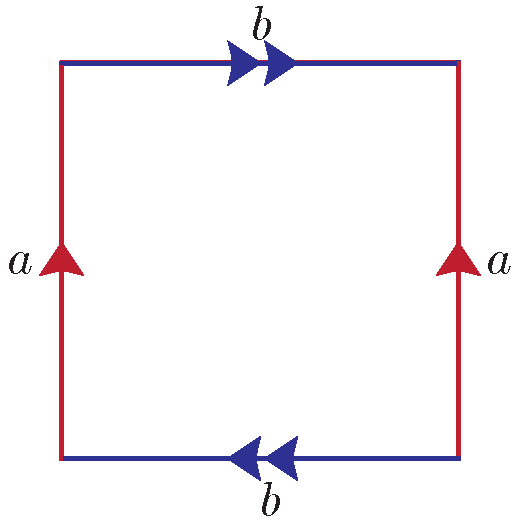
\includegraphics[trim=0cm 0cm 0cm 0cm, clip, scale=0.3]{images/klein.pdf}
		\end{center}
	\end{minipage}\\
	\begin{minipage}{.75\linewidth}
	Abbiamo visto inoltre come $P=\Proj^2\left(\R\right)$ ha un modello piano a due lati con parola $cc$.
\end{minipage}
\begin{minipage}{.24\linewidth}
	\begin{center}
		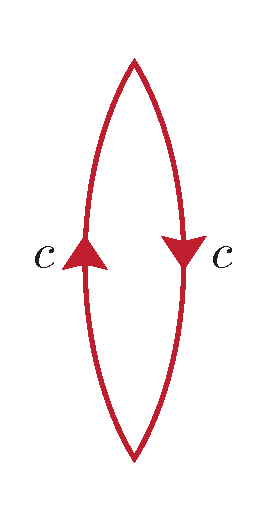
\includegraphics[trim=0cm 0cm 0cm 0cm, clip, scale=0.3]{images/proj2lines.pdf}
	\end{center}
\end{minipage}\\
	\begin{minipage}{.75\linewidth}
	Pertanto, per le osservazioni precedenti, la somma connessa di due piani proiettivi $P\# P$ ha il modello piano dato dalla parola $ccdd$.
\end{minipage}
\begin{minipage}{.24\linewidth}
	\begin{center}
		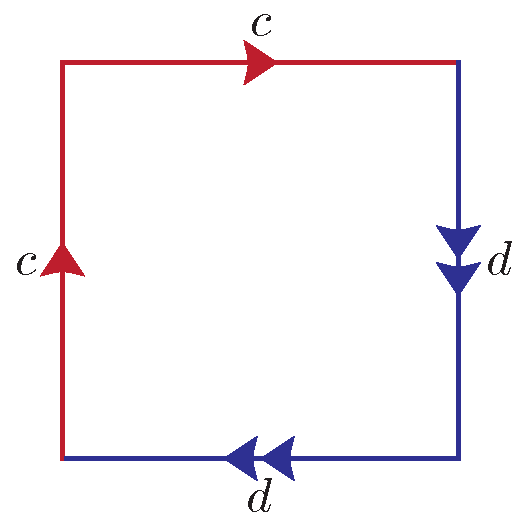
\includegraphics[trim=0cm 0cm 0cm 0cm, clip, scale=0.3]{images/projdouble.pdf}
	\end{center}
\end{minipage}\\
Vogliamo vedere che $aba^{-1}b$ e $ccdd$ danno la stessa superficie. Partiamo dal primo modello e tagliamo lungo la diagonale:
\begin{center}
	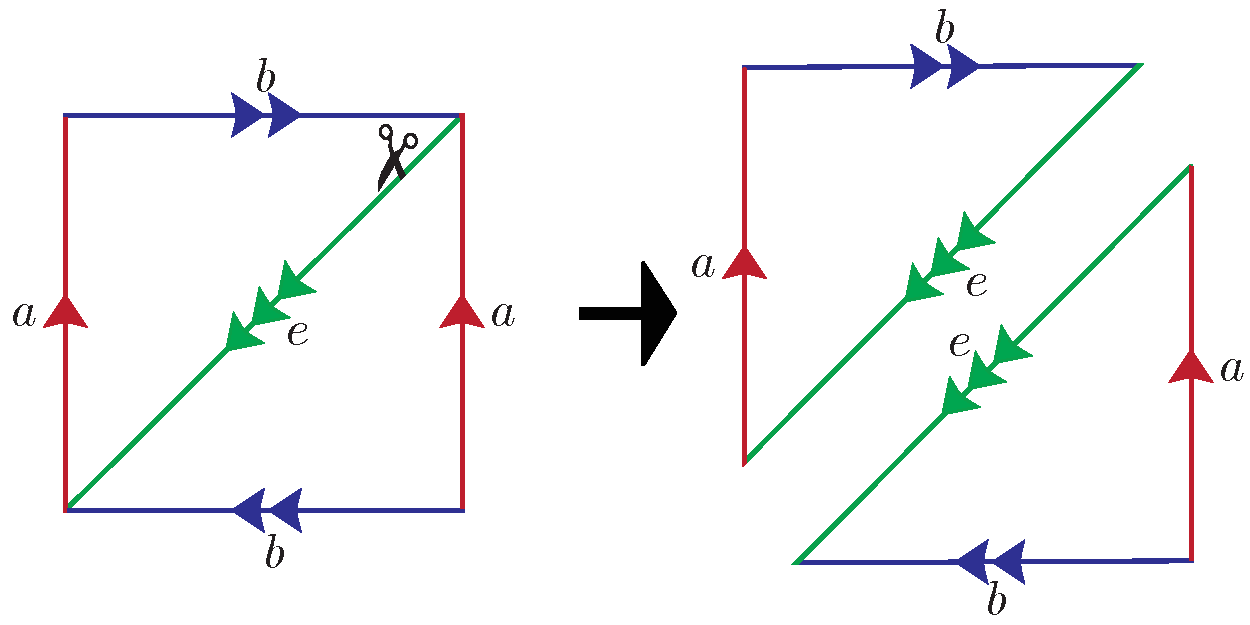
\includegraphics[trim=0cm 0cm 0cm 0cm, clip, scale=0.3]{images/kleintoprojdouble1.pdf}
\end{center}
Incolliamo lungo il lato $b$:
\begin{center}
	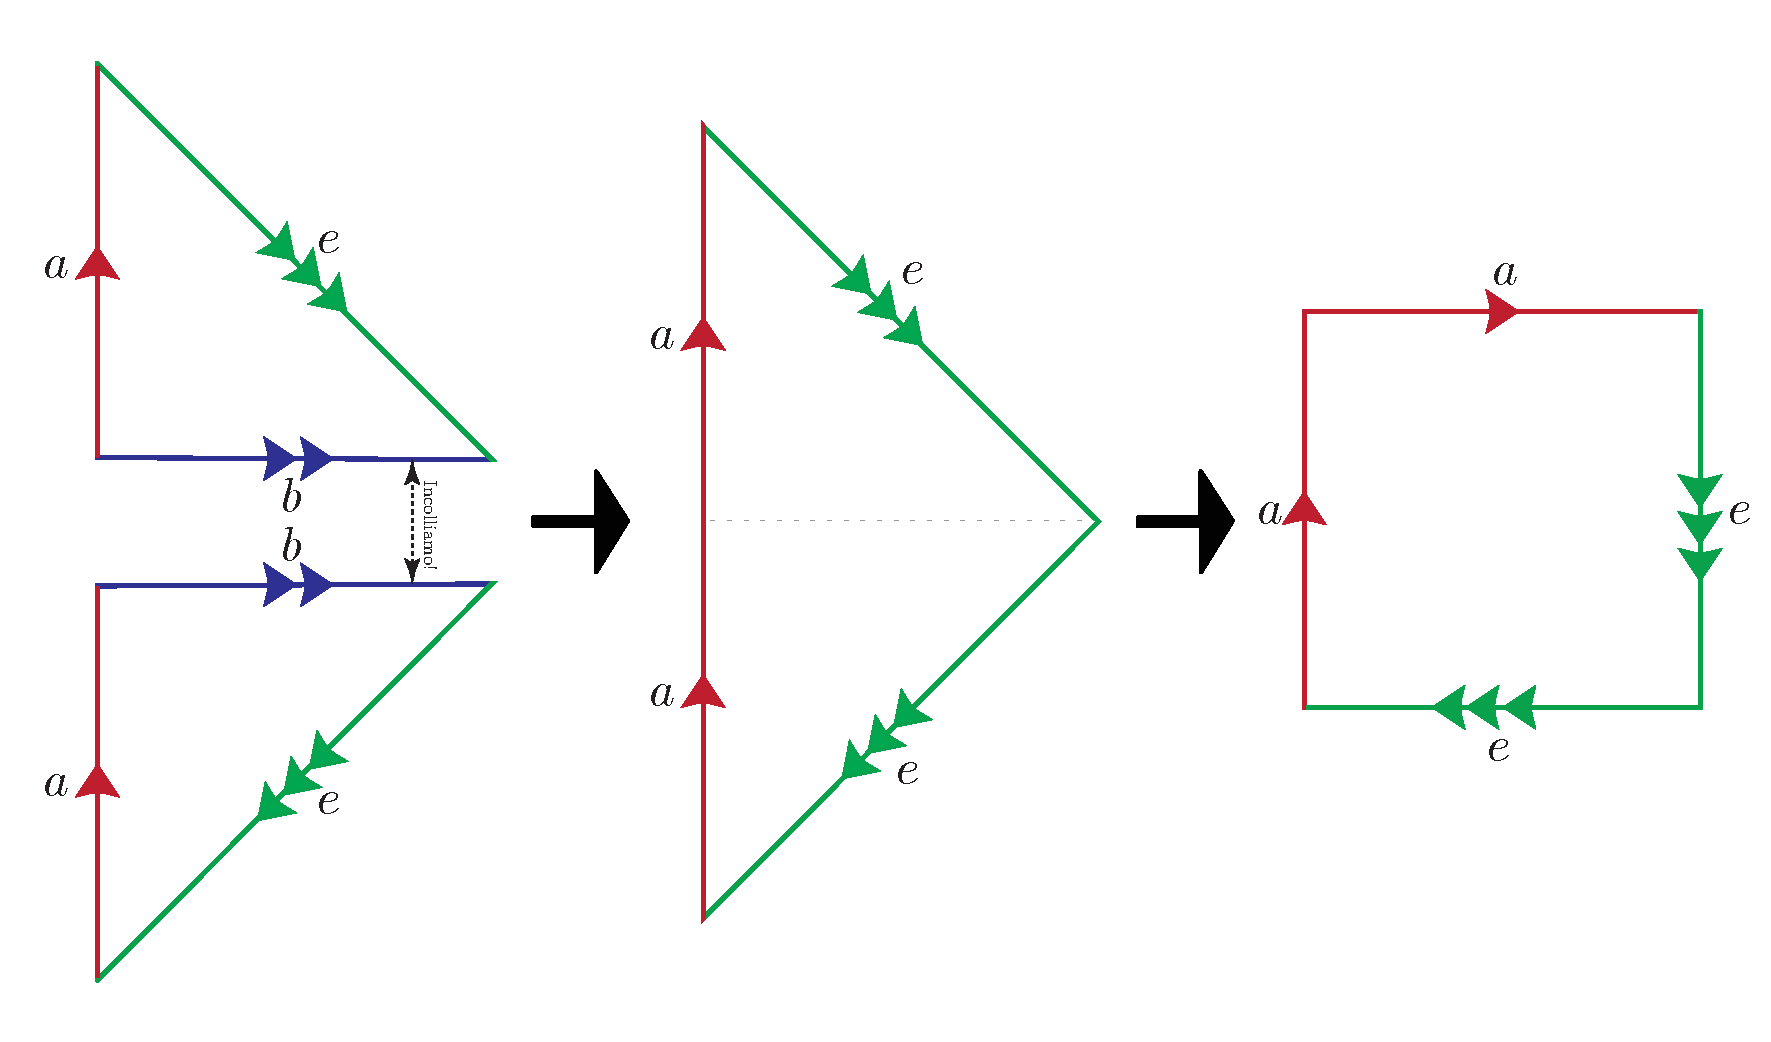
\includegraphics[trim=0cm 0cm 0cm 0cm, clip, scale=0.3]{images/kleintoprojdouble2.pdf}
\end{center}
Infatti, otteniamo come modello $aaee$, che corrisponde a $P\# P$.
\end{remark}
\begin{lemma}{n}[Somma connessa toro-piano proiettivo e bottiglia di Klein-piano proiettivo.]
	\begin{equation*}
		T\# P= K\# P=P\# P\# P
	\end{equation*}
\end{lemma}
\begin{proof}{n}
	Sappiamo già che, essendo $K=P\# P$, allora $K\# P=P\# P\# P$. Vogliamo invece mostrare ora che $T\# P$ sia uguale a $K\# P$. Facciamo un procedimento di taglia e incolla, partendo da $T\# P$, modello piano con parola $aba^{-1}b^{-1}cc$:
	\begin{center}
			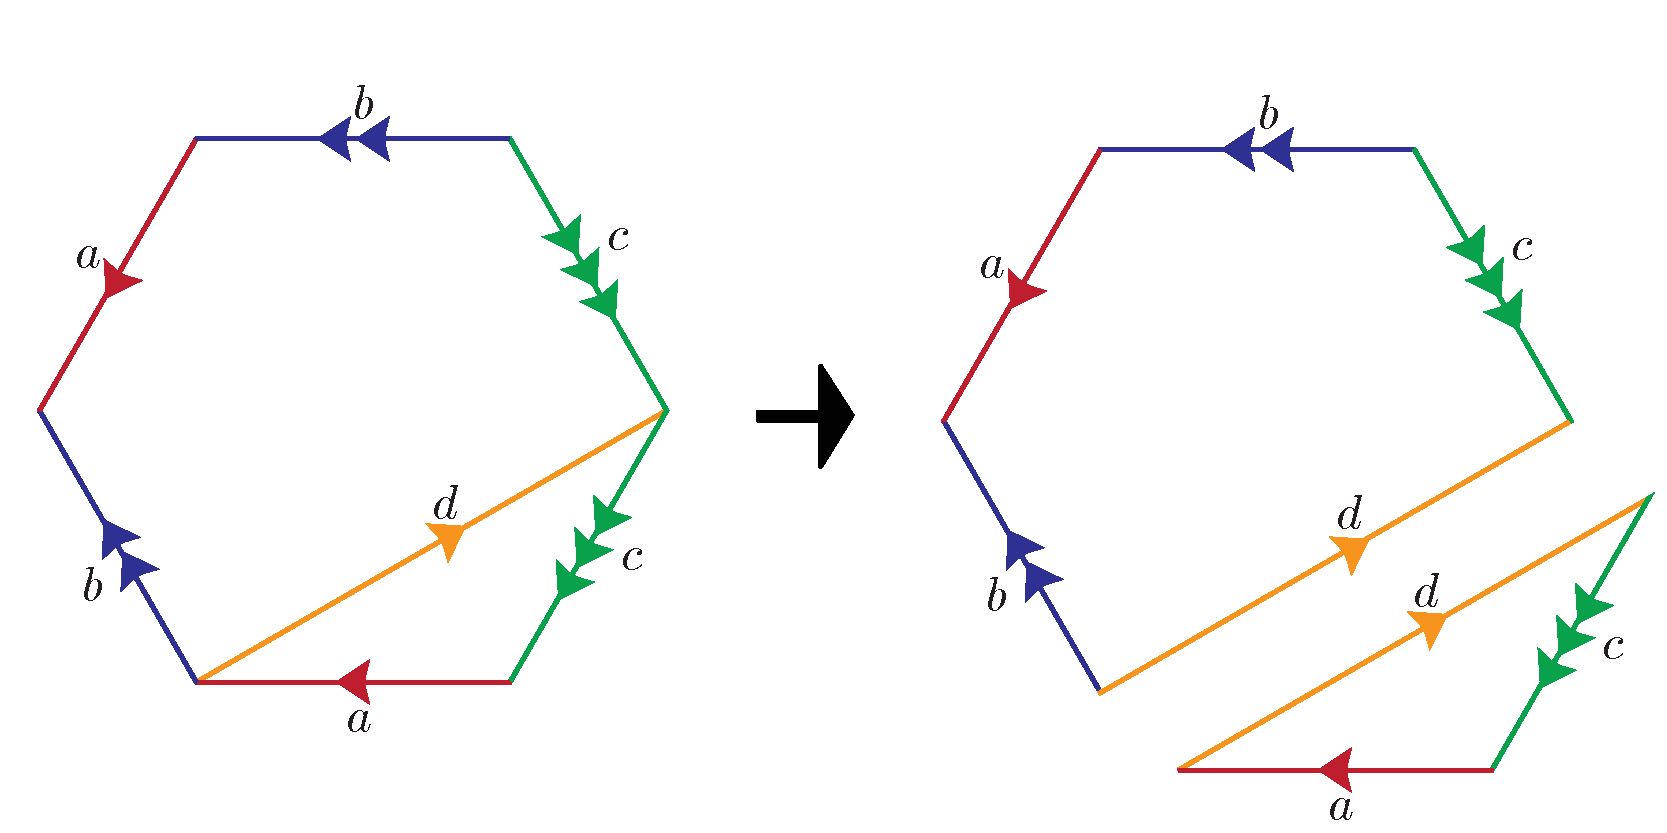
\includegraphics[trim=0cm 0cm 0cm 0cm, clip, scale=0.3]{images/torusplusproj1.pdf}
	\end{center}
Incolliamo lungo $c$:
\begin{center}
	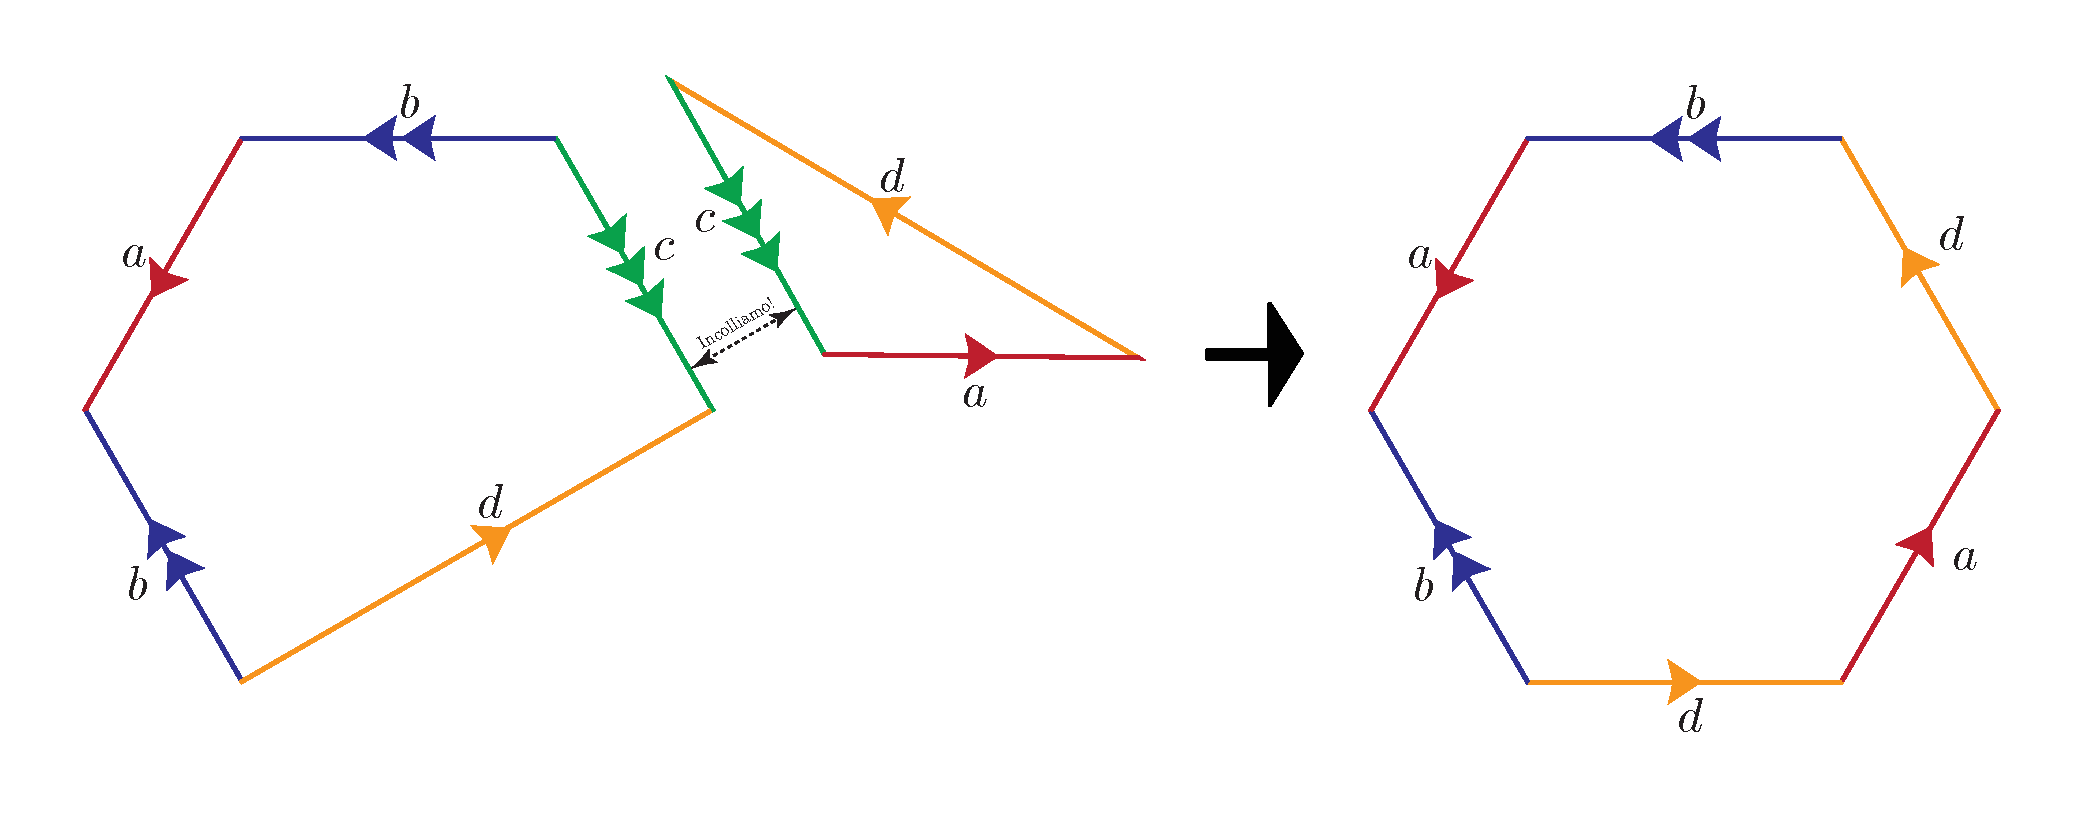
\includegraphics[trim=0cm 0cm 0cm 0cm, clip, scale=0.3]{images/torusplusproj2.pdf}
\end{center}
Otteniamo un modello piano di $T\# P$ che può essere descritto dalla parola $dadbab^{-1}$.\\
Prendiamo adesso $K\# P$, di parola $\underbrace{\delta\beta\delta^{-1}\beta}_{K}\underbrace{\gamma\gamma}_{P}$:
\begin{center}
	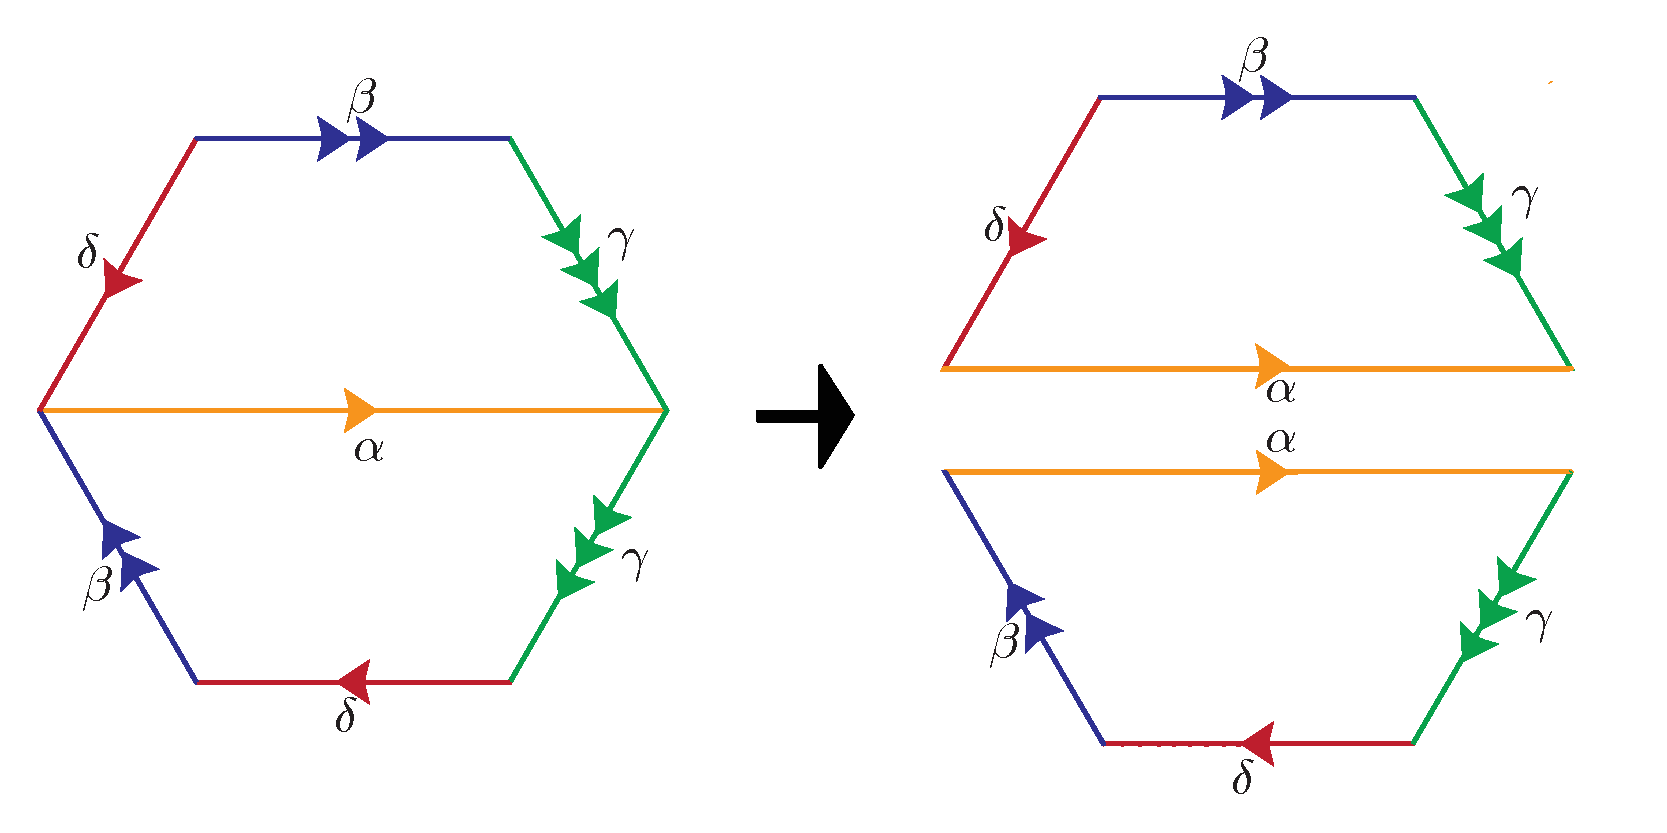
\includegraphics[trim=0cm 0cm 0cm 0cm, clip, scale=0.3]{images/kleinplusproj1.pdf}
\end{center}
Incolliamo lungo $\gamma$:
\begin{center}
	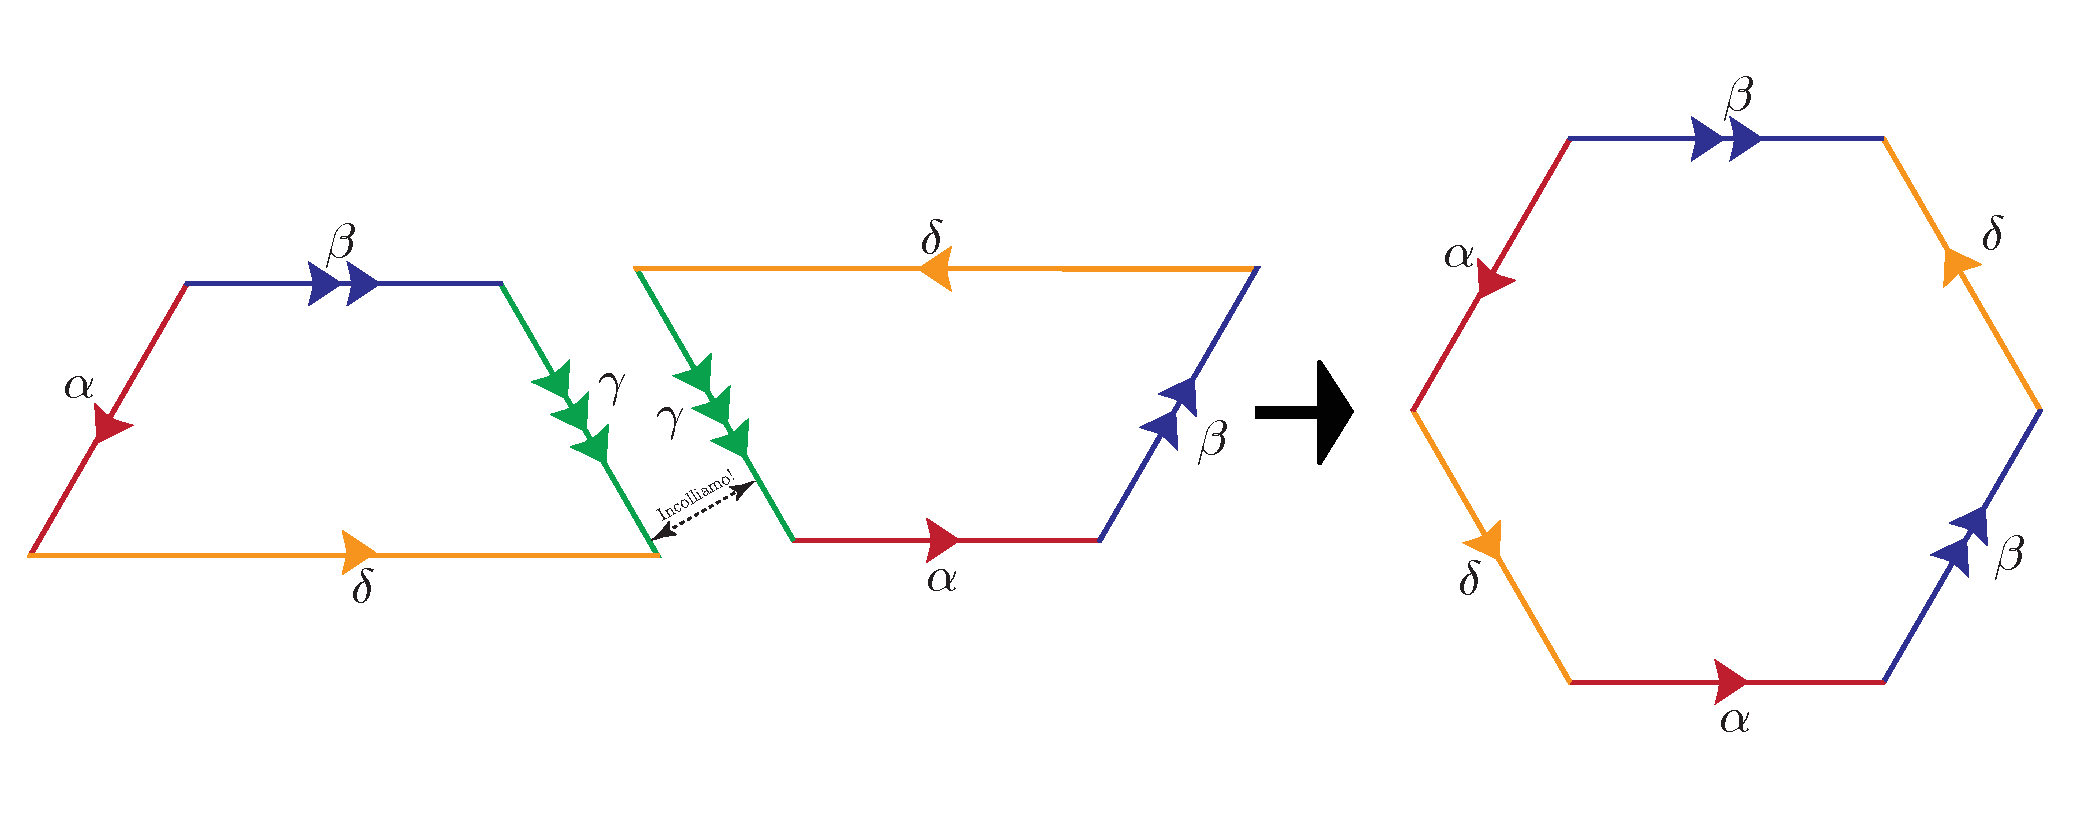
\includegraphics[trim=0cm 0cm 0cm 0cm, clip, scale=0.3]{images/kleinplusproj2.pdf}
\end{center}
Otteniamo un modello piano di $K\# P$ che può essere descritto dalla parola $\delta \alpha \delta\beta\alpha\beta^{-1}$, che corrisponde lettera per lettera al modello $T\# P$.\qedhere
\end{proof}
\begin{corollary}{}[Somma connessa tori-piani proiettivi]\label{toropiupiano}
Se $g\geq 1$ e $n\geq 1$, si ha
\begin{equation*}
	T_g\# P_n=P_{n+2g}.
\end{equation*}
\end{corollary}
\begin{proof}{n}
	Se $g=1$:
	\begin{equation*}
		T\# P_n=\underbrace{T\# P}_{P_3}\# P_{n-1}=P_3\# P_{n-1}=P\# P_{n+2}
	\end{equation*}
Procediamo per induzione su $g$; se è vero per $g-1$, allora:
\begin{equation*}
	T_g\# P_n=T\# T_{g-1}\# P_n=T\# P_{n+2g-2}=T\# P\# P_{n+2g-3}=P_3\# P_{n+2g-3}=P_{n+2g}\qedhere
\end{equation*}
\end{proof}
\section{Classificazione delle superfici topologiche compatte}
\begin{theorem}{}[Classificazione delle superfici topologiche compatte]\label{classificazionesuperficicompatte}
Ogni superfici topologica compatta è omeomorfa a $S^2$, $T_g$ per qualche $g\geq 1$ oppure $P_n$ per qualche $n\geq 1$. Inoltre, tali superfici sono tutte distinte, ovvero:
\begin{itemize}
	\item $T_g\ncong T_{g'}$ se $g\neq g'$.
	\item $P_n\ncong P_{n'}$ se $n\neq n'$.
	\item $T_g\ncong P_{n}\ \forall n\geq 1,\ \forall g\geq 1$.
	\item $S^2\ncong T_g\ \forall g\geq 1$.
	\item $S^2\ncong P_n\ \forall n\geq 1$.
\end{itemize}
\end{theorem}
Per la dimostrazione del teorema abbiamo bisogno di definire cos'è una \textit{triangolazione}.
\subsection{Triangolazione}
\begin{definition}{}[Triangolo geometrico]
	Sia $S$ una superficie compatta. Un \textbf{triangolo geometrico}\index{triangolo geometrico} $T$ in $S$ è un'applicazione
	\begin{equation*}
		\funct{}[\phi]{T'}{T\subseteq S},
	\end{equation*}
dove $T'\subseteq \R^2$ è un triangolo \textit{non} degenere (compreso dell'interno), inteso nel senso tradizionale del termine, mentre $\phi$ è un omeomorfismo. I \textbf{vertici} e i \textbf{lati} di $T$ sono le immagini tramite $\phi$ dei vertici dei lati di $T'$.
\begin{center}
	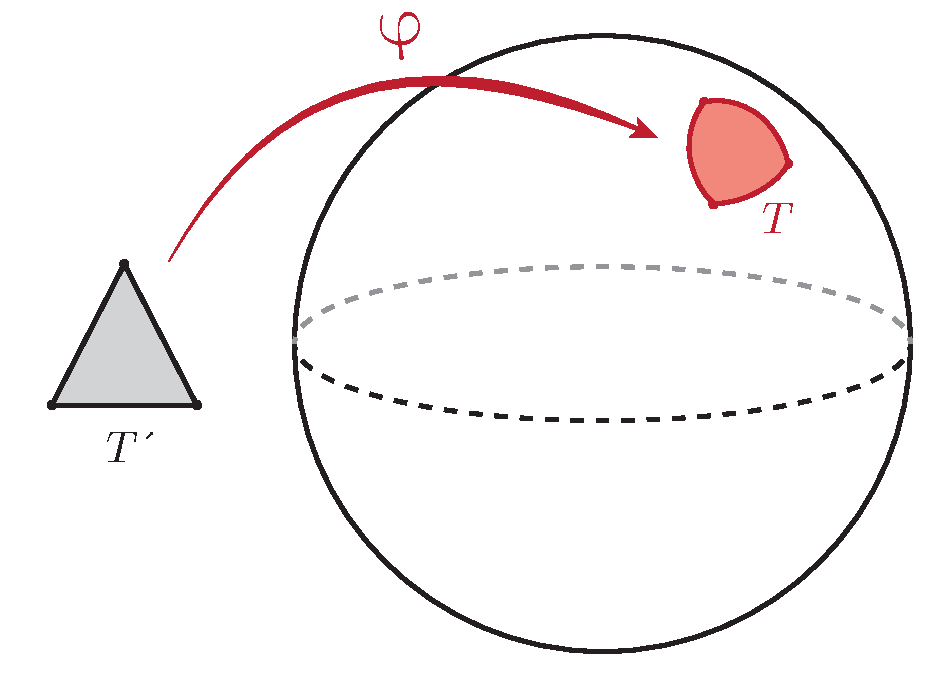
\includegraphics[trim=0cm 0cm 0cm 0cm, clip, scale=0.3]{images/spheretriangle.pdf}
\end{center}
\end{definition}
\begin{definition}{}[Triangolazione]
	Sia $S$ una superficie compatta. Una \textbf{triangolazione}\index{triangolazione} di $S$ è una collezione \textit{finita} di triangoli geometrici $T_1,\ \ldots,\ T_r$ in $S$ tale che:
	\begin{enumerate}
		\item $S=T_1\cup \ldots \cup T_r$.
		\item $\forall i\neq j$ si ha che $T_i\cap T_j$ può essere una di queste tre possibilità:
		\begin{itemize}
			\item $\emptyset$;
			\item un \textit{vertice} di entrambi i triangoli;
			\item un \textit{lato} di entrambi i triangoli.
		\end{itemize}
	\end{enumerate}
Una superficie compatta $S$ si dice \textbf{triangolabile}\index{triangolabilità} se ammette una triangolazione.
\end{definition}
\begin{example}{n}
	Il \textbf{tetraedro} dà una triangolazione della sfera con $4$ triangoli.
\end{example}
Enunciamo ora un teorema, di cui \textit{non} daremo dimostrazione, che ci servirà successivamente per poter classificare le superfici compatte direttamente con i loro modelli piani associati.
\begin{theorem}{q}[Teorema di Radò, 1925]
	Ogni superficie compatta è triangolabile.\qedhere
\end{theorem}
\begin{corollary}{n}[Ogni superficie compatta $S$ ha un modello piano]
\end{corollary}
\begin{proof}{n}
	Per il teorema di Radò, $S$ ammette una triangolazione $T_1,\ \ldots,\ T_r$. Riportiamo gli $r$ triangoli nel piano, con i lati identificati. Incolliamo poi i lati uno ad uno fino ad ottenere un unico poligono con delle identificazioni sui lati.\qedhere
\end{proof}
\subsection{Dimostrazione del teorema di classificazione: prima parte}
La prima parte della dimostrazione del teorema di classificazione si occupa di dimostrare che \textit{tutte le superfici compatte sono omeomorfe a $S^2$, $T_g$ o $P_n$}. Grazie al corollario appena dimostrato, possiamo studiare direttamente il \textit{modello piano} associato alla superficie compatta $S$ in esame, cioè studieremo un \textit{poligono} con i lati identificati a $2$ a $2$. Diamo una nomenclatura utile.
\begin{definition}{}[Coppie di lati]
	Nel modello piano, una \textit{coppia di lati} identificati tra di loro:
	\begin{itemize}
		\item è del \textbf{primo tipo} se, percorrendo il bordo del poligono, i due lati compaiono con \textit{orientazione opposta};
		\item è del \textbf{secondo tipo} se, percorrendo il bordo del poligono, i due lati compaiono con la \textit{stessa orientazione}.
	\end{itemize}
\end{definition}
\begin{example}{n}
	Nella \textit{bottiglia di Klein} $K$, modello con parola $aba^{-1}b$, i lati $a$ sono del I tipo, mentre i lati $b$ sono del II tipo.
\end{example}
La dimostrazione è \textit{costruttiva}: procederemo passo per passo, da un modello piano di una qualunque superficie compatta ad ottenere una delle superfici citate nel teorema con un \textbf{algoritmo di taglia e incolla}\index{algoritmo del taglia e incolla}.
\begin{proof}{}
\underbfsf{Passo 0:} se nel modello piano ci sono \textit{solo} $2$ lati abbiamo finito. Infatti, abbiamo solo due superfici con un modello di questo tipo, che abbiamo già visto:
\begin{center}
	\begin{minipage}{.19\linewidth}
		\begin{equation*}
			\begin{array}{cc}
				cc^{-1}\quad \text{(I tipo)}\\
				S=S^2
			\end{array}
		\end{equation*}
	\end{minipage}
	\begin{minipage}{.20\linewidth}
		\begin{center}
			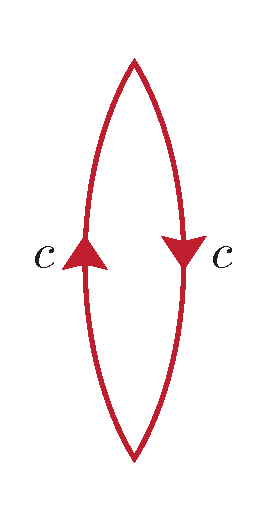
\includegraphics[trim=0cm 0cm 0cm 0cm, clip, scale=0.35]{images/sphere2lines.pdf}
		\end{center}
	\end{minipage}
	\begin{minipage}{.19\linewidth}
		\begin{equation*}
			\begin{array}{cc}
				cc\quad \text{(II tipo)}\\
				S=P
			\end{array}
		\end{equation*}
	\end{minipage}
	\begin{minipage}{.20\linewidth}
		\begin{center}
			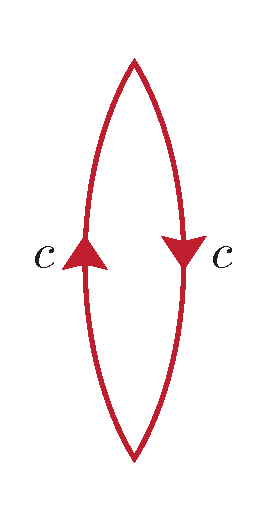
\includegraphics[trim=0cm 0cm 0cm 0cm, clip, scale=0.35]{images/proj2lines.pdf}
		\end{center}
	\end{minipage}
\end{center}
Possiamo supporre che nel modello piano c'è un numero di lati maggiore di $4$.\\
\underbfsf{Passo 1:} \textit{eliminazione delle coppie adiacenti del I tipo}.\\
Supponiamo che nel modello piano ci sia una coppia di lati \textit{adiacenti} del I tipo, come in figura:
\begin{center}
	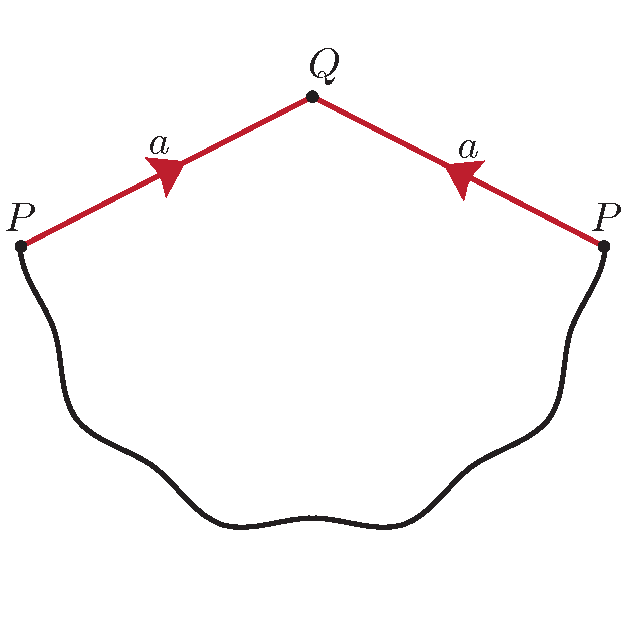
\includegraphics[trim=0cm 0cm 0cm 0cm, clip, scale=0.35]{images/cutandpastealgorithmstep1-1.pdf}
\end{center}
Incolliamo i lati $a$ della coppia; in questo modo, otteniamo un nuovo modello piano omeomorfo al primo con due lati in meno:
\begin{center}
	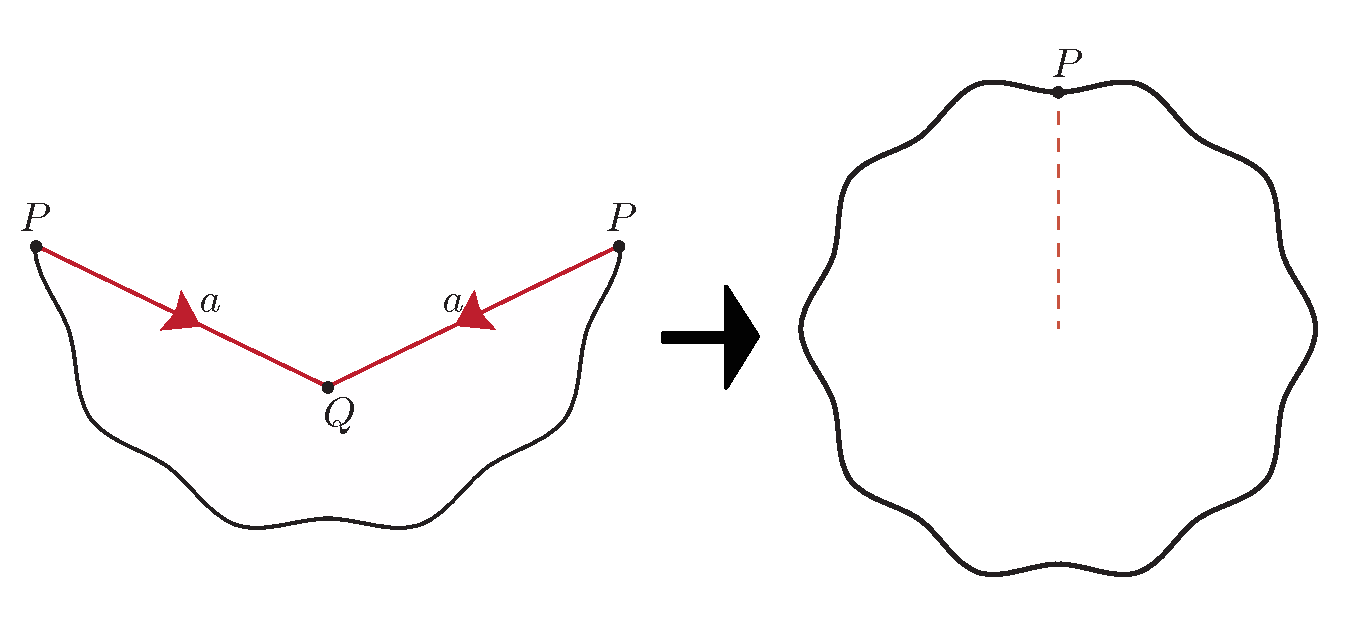
\includegraphics[trim=0cm 0cm 0cm 0cm, clip, scale=0.35]{images/cutandpastealgorithmstep1-2.pdf}
\end{center}
Ripetiamo il \underbfsf{passo 1} finché eliminiamo tutte le coppie adiacenti del I tipo. Se alla fine abbiamo due soli lati, ricadiamo nel \underbfsf{passo 0} e abbiamo già finito la dimostrazione.\\
\underbfsf{Passo 2:} \textit{riduzione dei vertici a un'unica classe di equivalenza}.\\
Supponiamo che i vertici del poligono \textit{non} siano tutti equivalenti. Dunque, esisterà un lato $b$ i cui due vertici $P$ e $Q$ \textit{non} sono equivalenti:
\begin{center}
	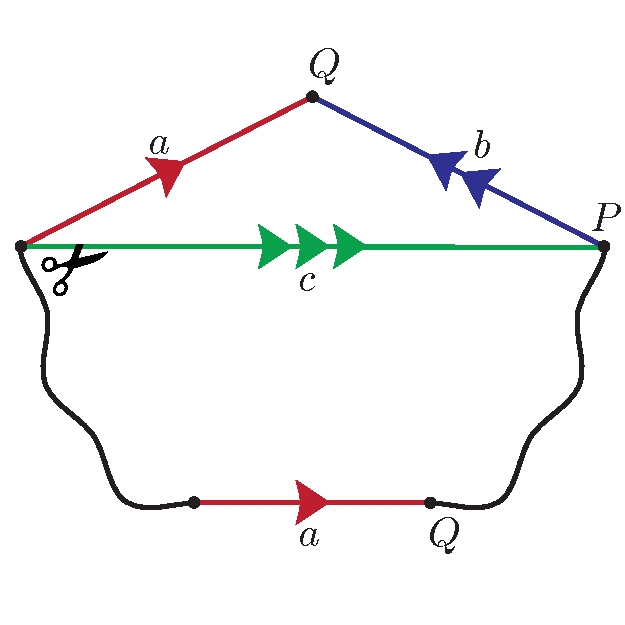
\includegraphics[trim=0cm 0cm 0cm 0cm, clip, scale=0.35]{images/cutandpastealgorithmstep2-1.pdf}
\end{center}
Consideriamo il secondo lato $a$ con vertice $Q$ e, facendo un taglio come in figura, incolliamo il lato $a$:
\begin{center}
	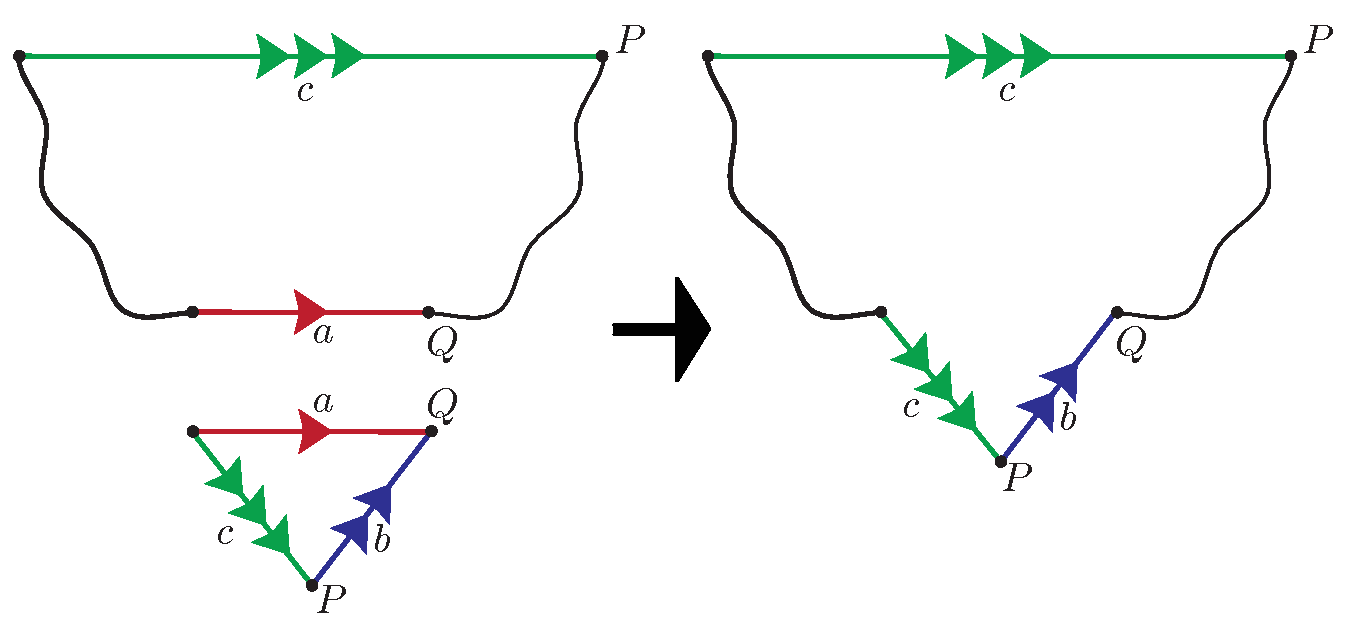
\includegraphics[trim=0cm 0cm 0cm 0cm, clip, scale=0.35]{images/cutandpastealgorithmstep2-2.pdf}
\end{center}
Abbiamo ora un vertice $Q$ \textit{in meno} e un vertice $P$ \textit{in più}. Ripetiamo questa operazione facendo via via diminuire i vertici $Q$. Quando rimane solo un vertice $Q$ deve essere parte di una coppia adiacente del I tipo; possiamo pertanto incollare il lato $a$ facendo scomparire il vertice $Q$. Alternando i \underbfsf{passi 1 e 2} arriviamo ad un modello piano con tutti i vertici identificati e senza coppie adiacenti del I tipo.\\
\underbfsf{Osservazione.} Quando incolliamo lungo una coppia di lati del I tipo \textit{non} ribaltiamo i lati, dunque le restanti coppie mantengono il tipo. Al contrario, quando invece incolliamo lungo una coppia di lati del II tipo, i lati restanti \textit{possono} cambiare tipo. Ad esempio, nel passo 2, se $a$ è del primo tipo (come nelle figure precedenti) anche il lato $c$ di taglio è del I tipo e le restanti coppie \textit{non} cambiano tipo. Invece, se $a$ è del II tipo, il lato $c$ è del II tipo:
	\begin{center}
		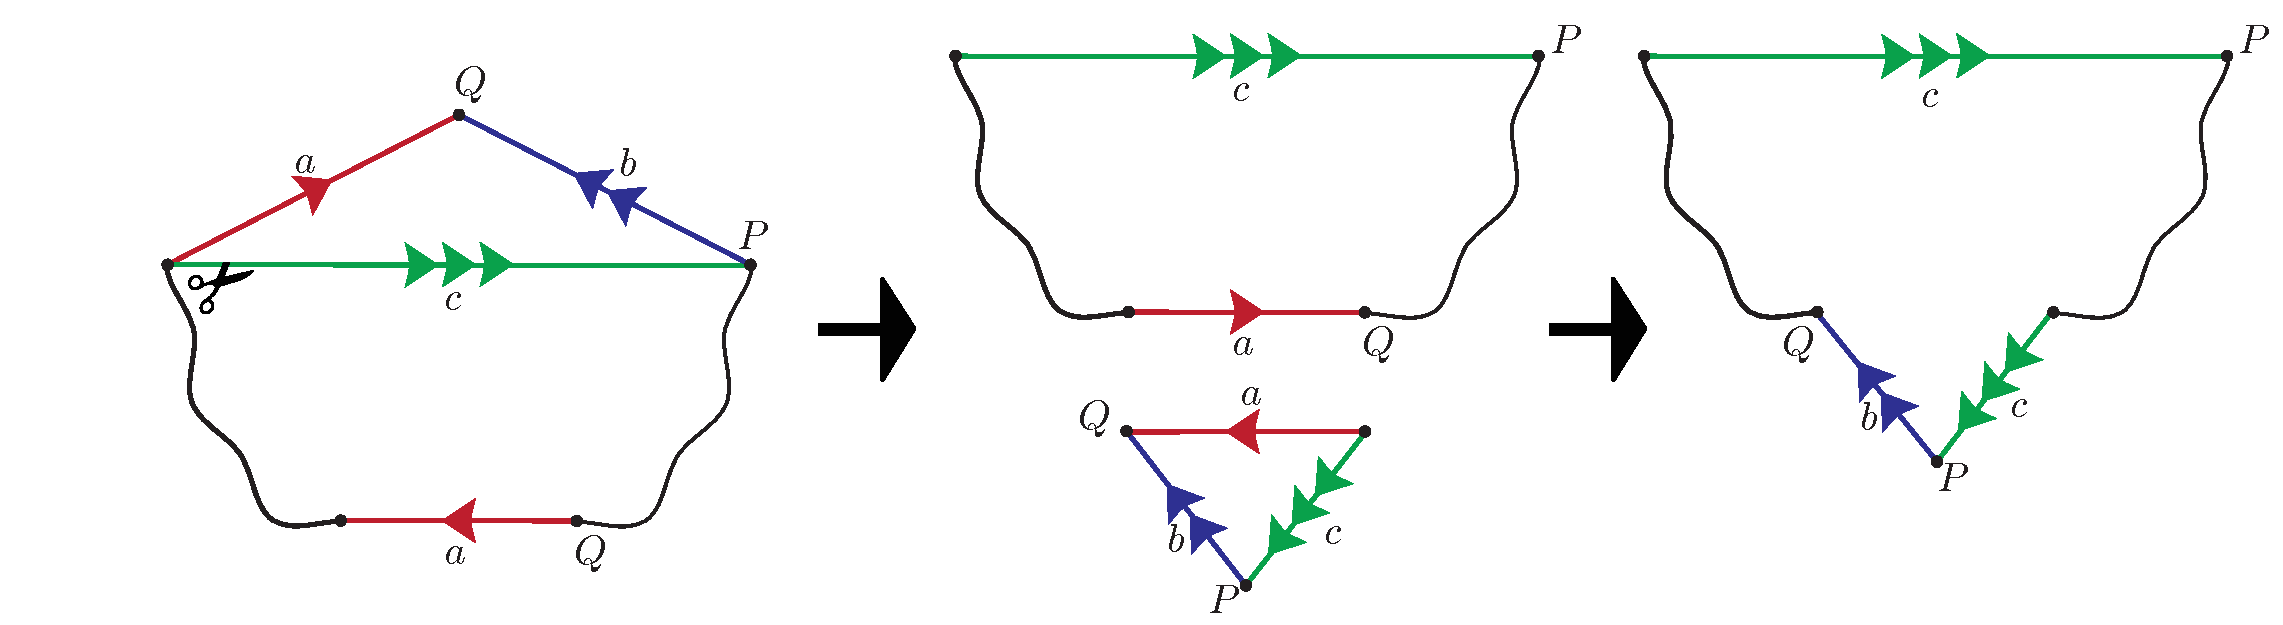
\includegraphics[trim=0cm 0cm 0cm 0cm, clip, scale=0.35]{images/cutandpastealgorithmstep2-3.pdf}
	\end{center}
In ogni caso, l'esistenza di \textit{almeno una} coppia di lati del II tipo è \textit{mantenuta} dal passo 2.\\
 \textit{Rendere adiacenti le coppie del II tipo}.\\
Supponiamo che ci sia una coppia di lati $a$ \textit{non} adiacenti del II tipo. Operiamo un taglio $b$ tra gli estremi finali della coppia e incolliamo la coppia stessa:
	\begin{center}
	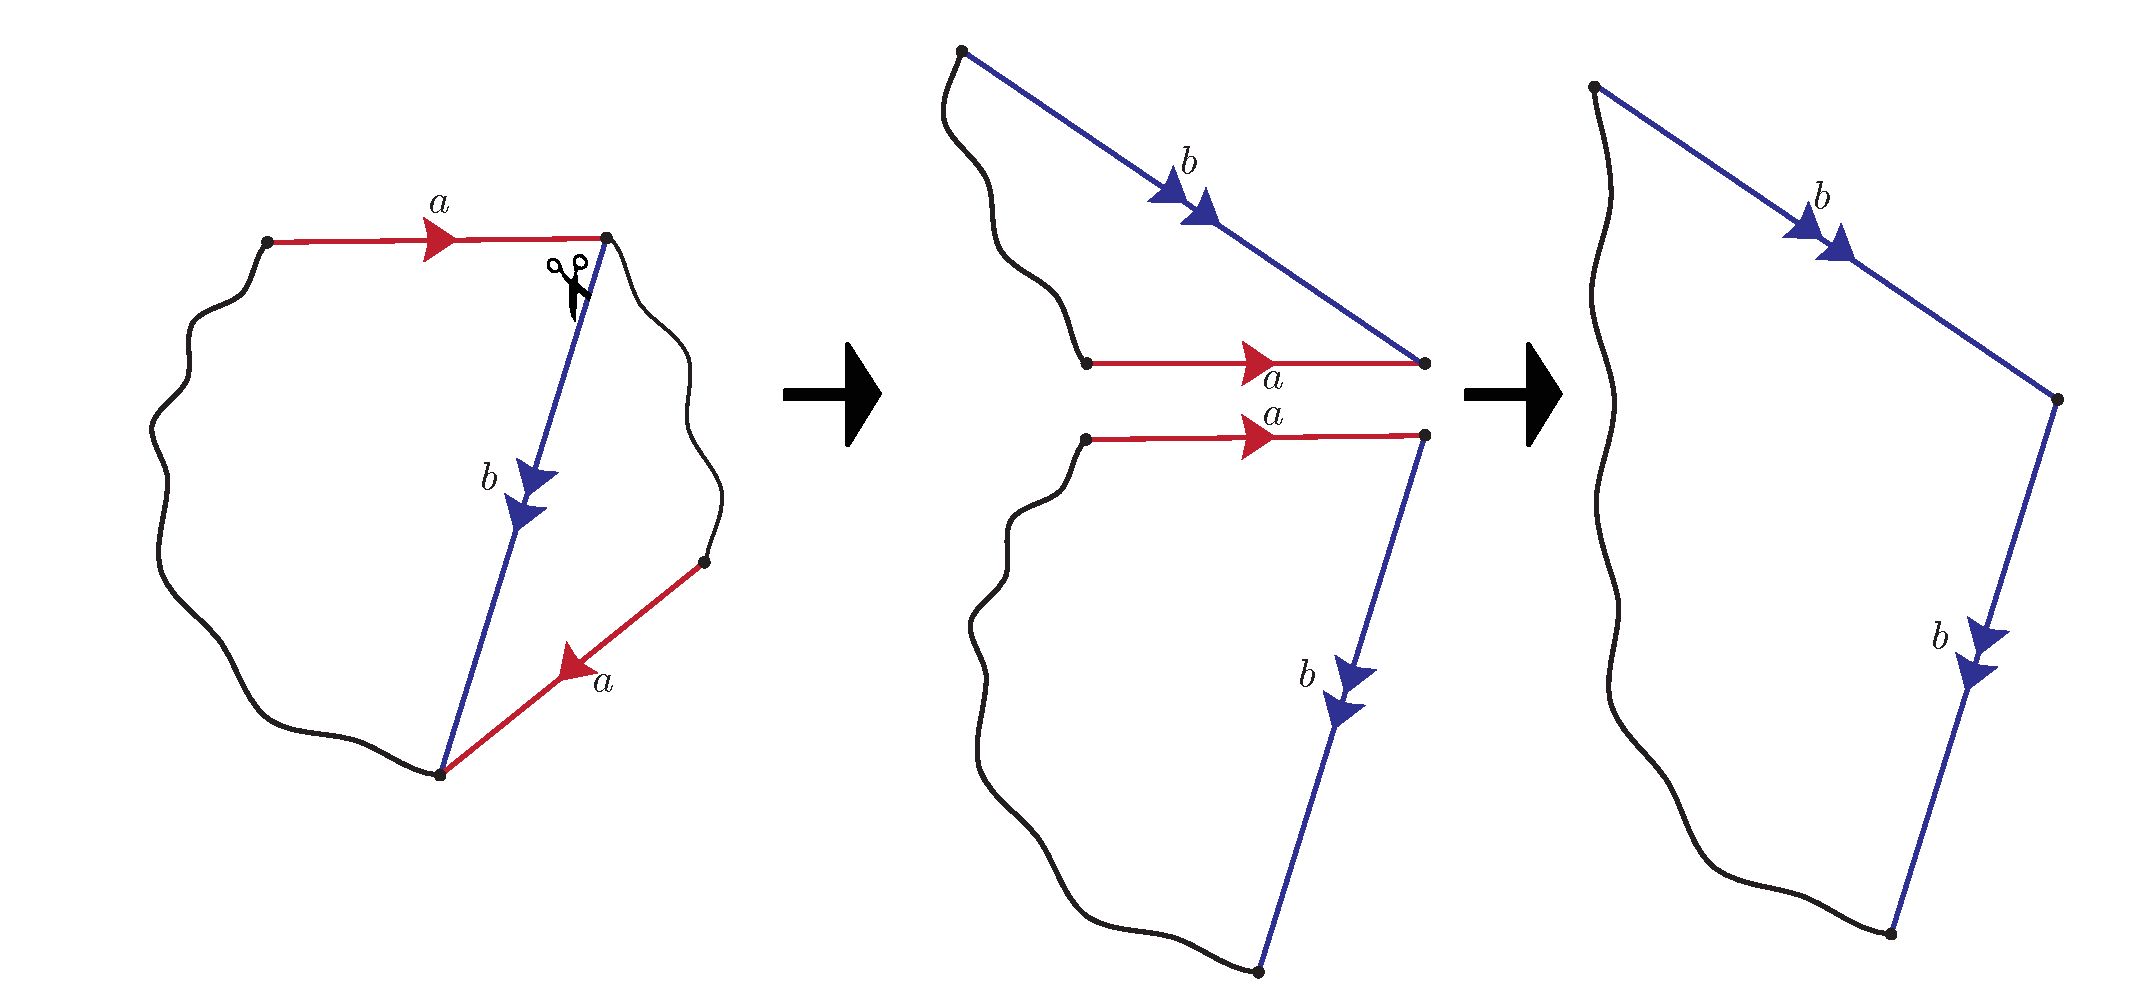
\includegraphics[trim=0cm 0cm 0cm 0cm, clip, scale=0.35]{images/cutandpastealgorithmstep3.pdf}
\end{center}
In questo modo rendiamo adiacenti tutte le coppie del II tipo.\\
Se ci sono solo \textit{coppie del II tipo}, abbiamo ottenuto una parola della forma
\begin{equation*}
	a_1a_1a_2a_2\ldots a_na_n \implies \ovaled{S\cong P_n}.
\end{equation*}
\underbfsf{Passo 4:} \textit{Raggruppare le coppie del I tipo}.\\
Supponiamo che nel modello piano ci sia almeno una coppia del primo tipo, non adiacente per i passi precedenti:
\begin{center}
	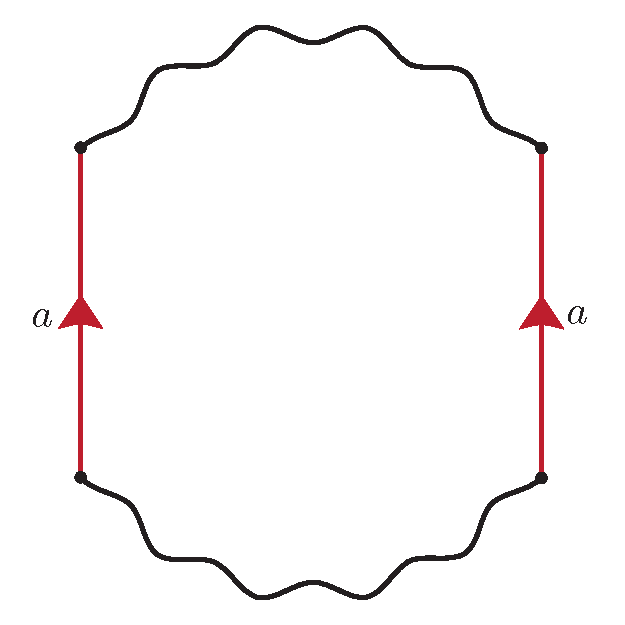
\includegraphics[trim=0cm 0cm 0cm 0cm, clip, scale=0.35]{images/cutandpastealgorithmstep4-1.pdf}
\end{center}
Allora deve esistere un'altra coppia di lati del I tipo tali che queste coppie si separino a vicenda. Infatti, i vertici sono tutti identificati tra loro, in particolare lo sono i due vertici di $a$. In altre parole, deve esistere un lato $b$ nella parte superiore identificato ad un lato $b$ nella parte inferiore:
	\begin{center}
	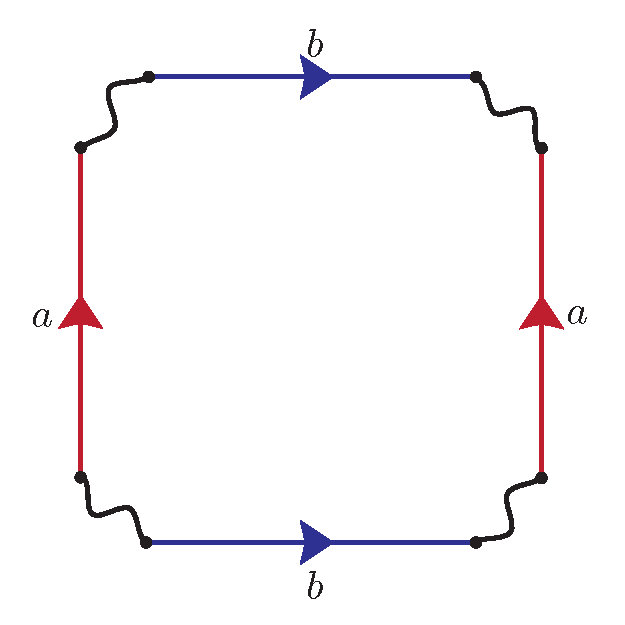
\includegraphics[trim=0cm 0cm 0cm 0cm, clip, scale=0.35]{images/cutandpastealgorithmstep4-2.pdf}
\end{center}
Siccome i lati $b$ \textit{non} sono adiacenti e abbiamo già reso adiacenti tutte le coppie di lati del II tipo, $b$ deve essere una coppia di lati del I tipo.
Operiamo due taglia e incolla per raggruppare le due coppie.
\begin{enumerate}
	\item[\underline{4.1}] Taglio un lato $c$ lungo gli estremi finali di $a$ nella stessa direzione di $b$ e incollo $b$:
	\begin{center}
		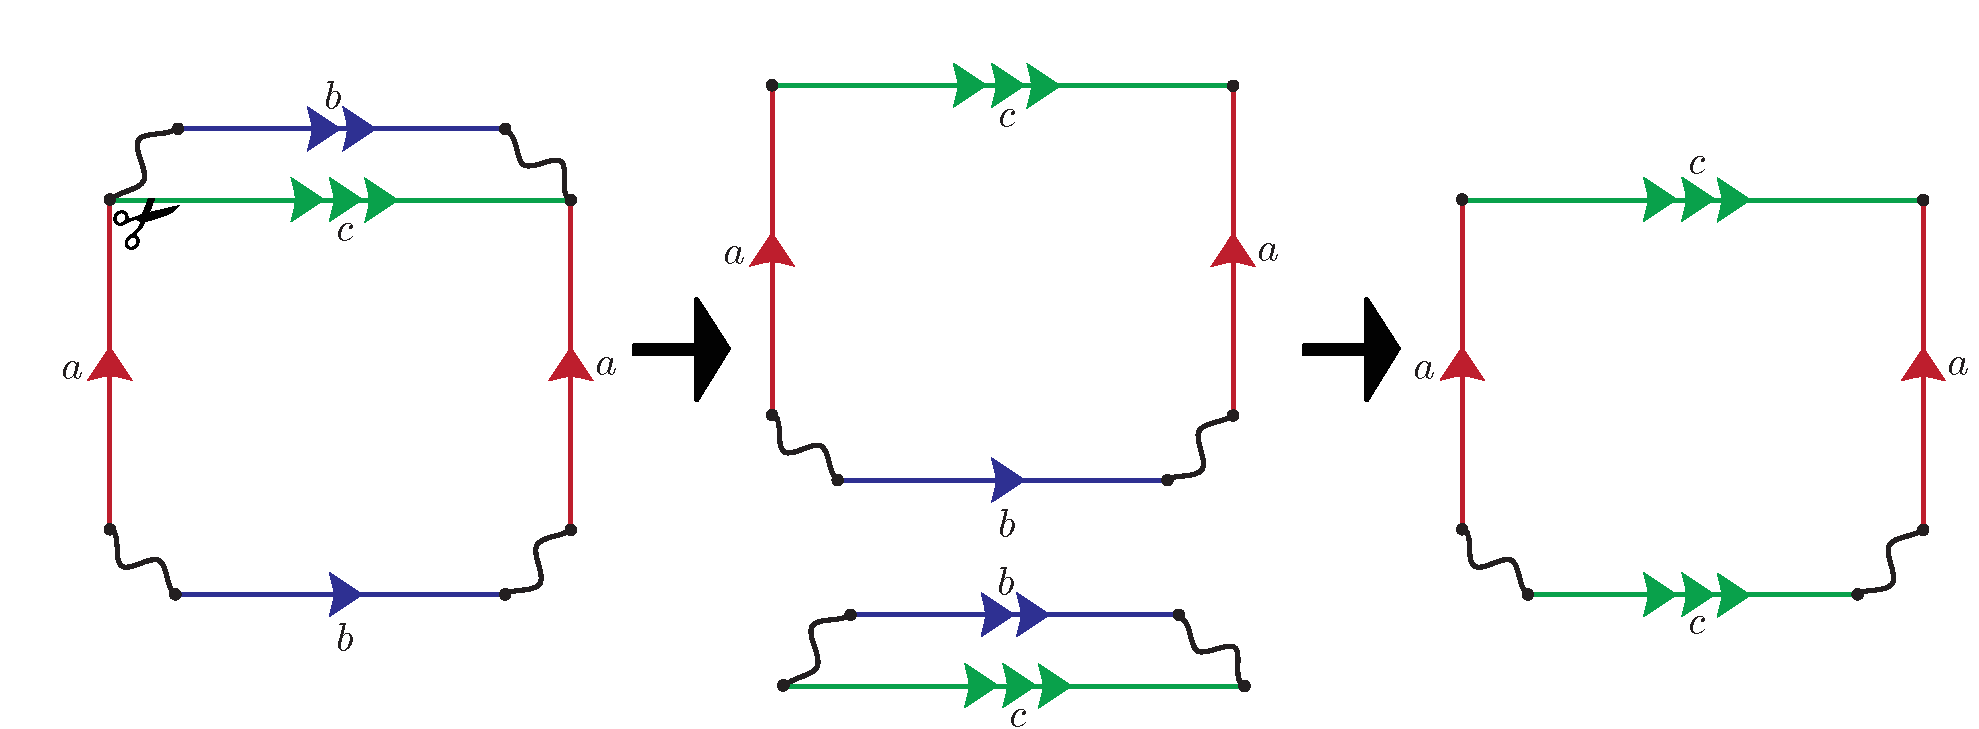
\includegraphics[trim=0cm 0cm 0cm 0cm, clip, scale=0.35]{images/cutandpastealgorithmstep4-3.pdf}
	\end{center}
	\item[\underline{4.2}] Taglio un lato $d$ lungo gli estremi finali di $c$ nella stessa direzione di $a$ e incollo $a$:
	\begin{center}
		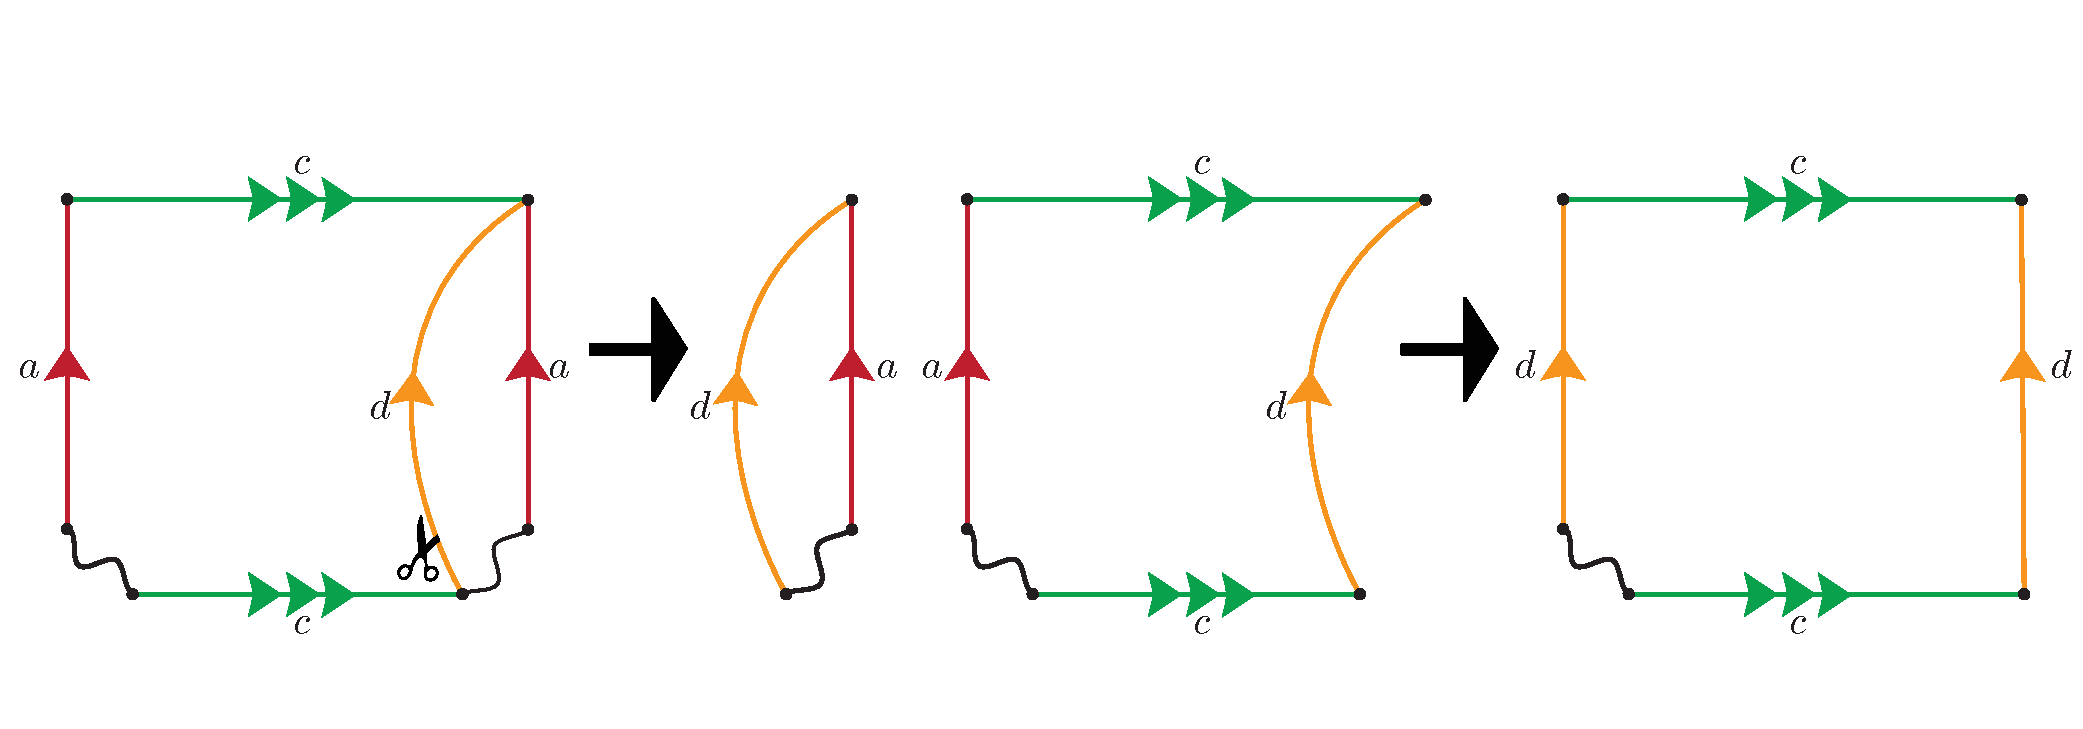
\includegraphics[trim=0cm 0cm 0cm 0cm, clip, scale=0.35]{images/cutandpastealgorithmstep4-4.pdf}
	\end{center}
\end{enumerate}
In queste operazioni incolliamo lungo coppie del I tipo, pertanto i tipi delle coppie \textit{non cambiano!}
\begin{itemize}
	\item Se nel modello piano compaiono \textit{solo} coppie del \textit{I tipo}, dopo un numero finito di passi otteniamo la parola
	\begin{equation*}
		a_1b_1a_1^{-1}b_1^{-1}a_2b_2a_2^{-1}b_2^{-1}\ldots a_nb_na_n^{-1}b_n^{-1}\implies \ovaled{S\cong T_g}.
	\end{equation*}
	\item Se invece nel modello piano compaiono sia coppie adiacenti del II tipo, sia sequenze $aba^{-1}b^{-1}$ di coppie del I tipo, allora $S$ è data dalla somma connessa di tori e piani proiettivi, con almeno un piano proiettivo, pertanto per il corollario \ref{toropiupiano} (pag. \pageref{toropiupiano}) segue che $\ovaled{S\cong P_n}$.\qedhere
\end{itemize}
\end{proof}
\begin{remark}{n}
	Si ottiene sempre un piano proiettivo se e solo nel modello iniziale c'è almeno una coppia di lati del II tipo perché i passi mantengono il tipo.
\end{remark}
\section{Orientabilità}
\begin{definition}{}[Nastro di Möbius]\label{nastromobius}
\begin{minipage}{.75\linewidth}
Definiamo il \textbf{nastro di Möbius} (aperto) $N_0\subseteq \R^3$ come lo spazio $\left[0,\ 1\right]\times (0,\ 1)$ (mentre si considera $\left[0,\ 1\right]\times [0,\ 1]$ nel caso chiuso $N$) con i lati quozientati come in figura.
	\end{minipage}
	\begin{minipage}{.14\linewidth}
		\begin{center}
			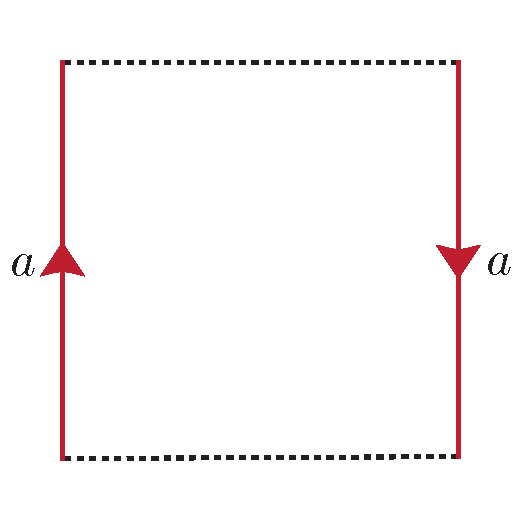
\includegraphics[trim=0cm 0cm 0cm 0cm, clip, scale=0.4]{images/openmoebius.pdf}
		\end{center}
	\end{minipage}
\end{definition}
\begin{remark}{n}
	$N_0$ è una superficie topologica, ma \textit{non} è compatta in quanto \textit{non} è chiusa.
\end{remark}
\begin{intuitively}{n}
	Immaginiamo di avere una \textit{figura bidimensionale} posta sulla sfera $S^2$; essa è libera di muoversi su di essa. Qualunque percorso chiuso essa faccia, la figura tornerà al punto di partenza \textit{esattamente come era partita}. Prendiamo invece il \textit{nastro di Möbius}. Dopo un percorso attorno al nastro, la figura torna al punto di partenza non com'era partita, bensì ci ritorna con la sua \textit{immagine speculare}! Oltre a questo strano avvenimento, notiamo che la figura nel caso della sfera percorre sempre e solo un percorso sull'esterno o sull'interno della sfera, ma \textit{mai} contemporaneamente su entrambi. Nel caso del nastro di Möbius, la figura percorre l'\textit{intera superficie} in un unico percorso.\\
	In questi termini, diciamo che la sfera è una superficie \textbf{orientabile}: non esistono percorsi che mi ribaltano una figura piana su di essa e (vista come superficie in $\R^3$) ho due lati ben distinti, l'interno e l'esterno della sfera. Il nastro di Möbius, invece, \textbf{non è orientabile}: la figura si \textit{ribalta} e, allo stesso tempo, percorre tutta la superficie; in altre parole, non esiste un ‘‘interno'' o un ‘‘esterno'' del nastro.
\end{intuitively}
I comportamenti sul nastro di Möbius che abbiamo appena osservato si presentano anche in superfici come il \textit{piano proiettivo reale} o la \textit{bottiglia di Klein}; in particolare, si ha questo proprio perché possiamo identificare su di esse un percorso esattamente \textit{analogo} a quello visto sul nastro di Möbius. Possiamo formalizzare l'\textit{orientabilità} utilizzando questo principio.
\begin{definition}{}[Orientabilità]
	Una superficie topologica si dice \textbf{orientabile}\index{orientabilità} se \textit{non} contiene un sottospazio omeomorfo al nastro di Möbius (aperto o chiuso). Altrimenti $S$ si dice \textbf{non orientabile}.
\end{definition}
\begin{example}{pn}~{}
	\begin{itemize}
		\item $N_0$ \textit{non} è orientabile.
		\item $P=\Proj^2\left(\R\right)$ \textit{non} è orientabile:
		\begin{center}
			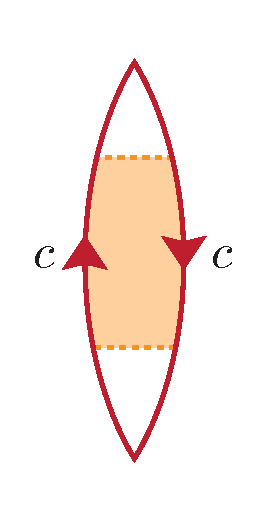
\includegraphics[trim=0cm 0cm 0cm 0cm, clip, scale=0.35]{images/projmoebius.pdf}
		\end{center}
		\item $K$ \textit{non} è orientabile:
		\begin{center}
			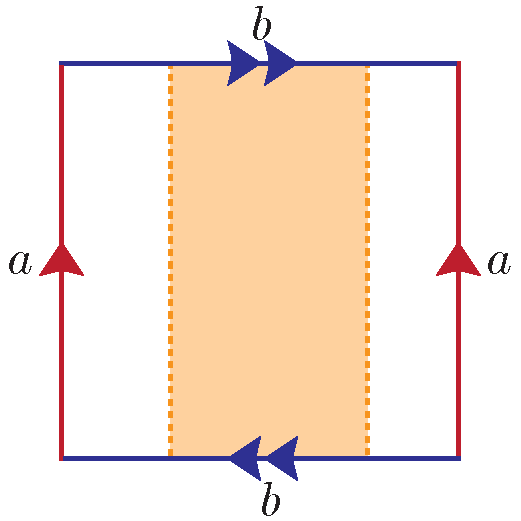
\includegraphics[trim=0cm 0cm 0cm 0cm, clip, scale=0.35]{images/kleinmoebius.pdf}
		\end{center}
	\item Una superficie il cui modello piano contiene una coppia di lati del II tipo \textit{non} è orientabile:
	\begin{center}
		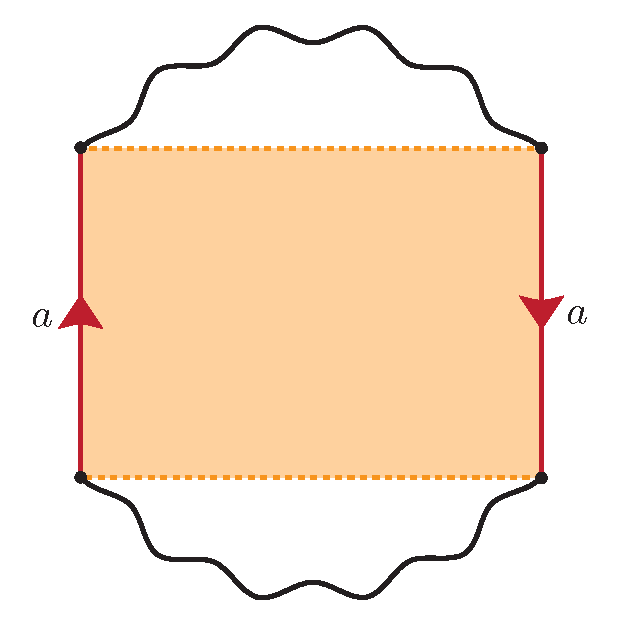
\includegraphics[trim=0cm 0cm 0cm 0cm, clip, scale=0.35]{images/generalmoebius.pdf}
	\end{center}
	\end{itemize}
\end{example}
\begin{remark}{n}~{}
	\begin{enumerate}
		\item $S^2$ e $T_g$ sono orientabili $\forall g\geq 1$.
		\item Se una superficie \textit{compatta} è omeomorfa a un sottospazio di $\R^3$, allora è \textit{orientabile} ed è rappresentabile.
	\end{enumerate}
\end{remark}
\begin{remark}{n}
	L'\textbf{orientabilità} è una proprietà topologica, cioè è invariante per omeomorfismi.
\end{remark}
\subsection{Dimostrazione del teorema di classificazione: seconda parte}
Noto ciò, con il concetto di orientabilità possiamo fare un passettino avanti nella classificazione delle superfici.
\begin{corollary}{nq}[Sfera, tori e piani proiettivi non sono omeomorfi]~{}
	\begin{align*}
		S^2 &\ncong P_n\ \forall n\geq 1\\
		T_g &\ncong P_n\ \forall n\geq 1,\ \forall g\geq 1\qedhere
	\end{align*}
\end{corollary}
\begin{corollary}{}[Orientabile se e solo se il modello piano non ha lati del II tipo]
	Sia $S$ una superficie compatta con un suo modello piano. Allora $S$ è \textit{orientabile} se e solo se il modello \textit{non} contene coppie di lati del II tipo.
\end{corollary}
\begin{proof}{n}~{}\\
$\rightimplies$Se c'è una coppia di lati del II tipo, costruiamo facilmente un nastro di Möbius collegandone gli estremi.\\
$\leftimplies$Applicando l'algoritmo del taglia e incolla, se non ci sono lati del II tipo otteniamo una superficie omeomorfa a $S^2$ o a $T_g$, entrambe superfici orientabili.\qedhere
\end{proof}
\section{Suddivisione di una superficie compatta}
\begin{definition}{}[Lato]
	Un \textbf{lato}\index{lato} in $S$ superficie compatta è un sottospazio $L\subseteq S$ con un'applicazione continua $\funct{}[f]{\unint}{L}$ tale che valga una delle due proprietà seguenti:
	\begin{itemize}
		\item $f$ è omeomorfismo tra $\unint$ e $L$;
		\item $f$ è iniettivo su $\left[0,\ 1\right)$, $f\left(0\right)=f\left(1\right)$ e $f$ induce un omeomorfismo tra $L$ e $S^1$, cioè $f$ è un'\textit{identificazione}.
	\end{itemize}
Definiamo come \textbf{vertici}\index{vertice} del lato, rispetto ai due casi sopra:
\begin{itemize}
	\item $f\left(0\right)$ e $f\left(1\right)$;
	\item $f\left(0\right)$.
\end{itemize}
\end{definition}
\begin{definition}{}[Suddivisione di una superficie compatta]
	Una \textbf{suddivisione}\index{suddivisione} $\mathcal
	S$ di una superficie compatta $S$ è data da:
	\begin{itemize}
		\item un sottoinsieme finito $V$ di $S$, i cui punti sono detti \textbf{vertici};
		\item un insieme finito $L_1,\ \ldots,\ L_m$ in $S$ di lati;
	\end{itemize}
tali che:
\begin{enumerate}
	\item $\forall L$, $L_i\cap V=\left\{\text{vertici di }L_i\right\}$;
	\item $\forall i\neq j$, $L_i\cap L_j\subseteq V$;
	\item $S\setminus\left(L_1\cup\ldots\cup L_m\right)$ ha un numero \textit{finito} di componenti connesse dette \textbf{facce}\index{faccia} della suddivisione e ogni faccia è omeomorfa a un disco aperto di $\R^2$.
\end{enumerate}
\end{definition}	
\begin{example}{n}
	Una \textbf{triangolazione} $T_1,\ \ldots,\ T_r$ di $S$ induce \textit{sempre} una suddivisione, in cui:
	\begin{itemize}
		\item $V=$ vertici di $T_1,\ \ldots,\ T_r$.
		\item $L_1,\ \ldots,\ L_m=$ lati di $T_1,\ \ldots,\ T_r$.
		\item Facce $=$ interni di $T_1,\ \ldots,\ T_r$.
	\end{itemize}
Pertanto, ogni superficie compatta ammette almeno una suddivisione perché esiste sempre una triangolazione per il \textit{Teorema di Radò}.
\end{example}
\begin{example}{pn}~{}
	\begin{itemize}
		\item $S^2$ ha una suddivisione (ulteriore a quella data dal tetraedro) data da un \textcolor{redill}{\textbf{unico vertice}}, un \textcolor{greenill}{\textbf{unico lato}} e \textcolor{blueill}{\textbf{due facce}}.
			\begin{center}
				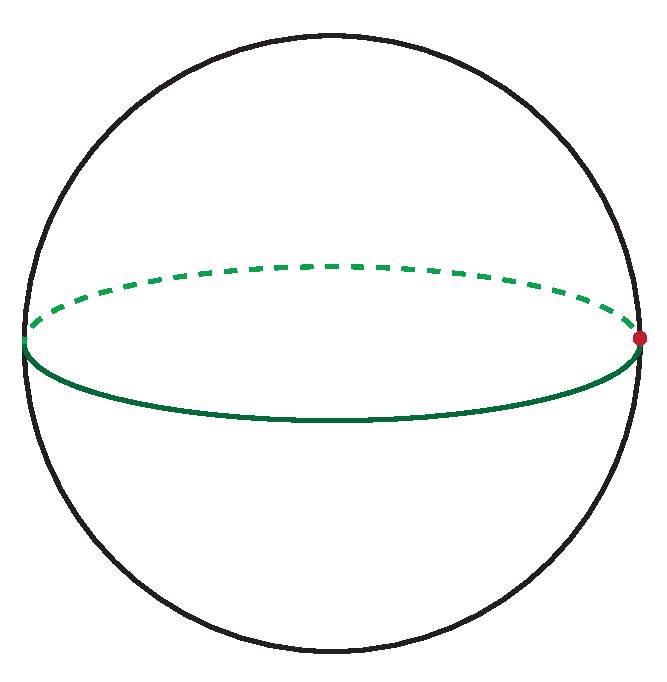
\includegraphics[trim=0cm 0cm 0cm 0cm, clip, scale=0.35]{images/spheresubdivision.pdf}
			\end{center}
		\item Il toro ha una suddivisione data da un \textcolor{redill}{\textbf{unico vertice}}, \textcolor{greenill}{\textbf{due lati}} e un'\textcolor{blueill}{\textbf{unica faccia}}.	
		\begin{center}
			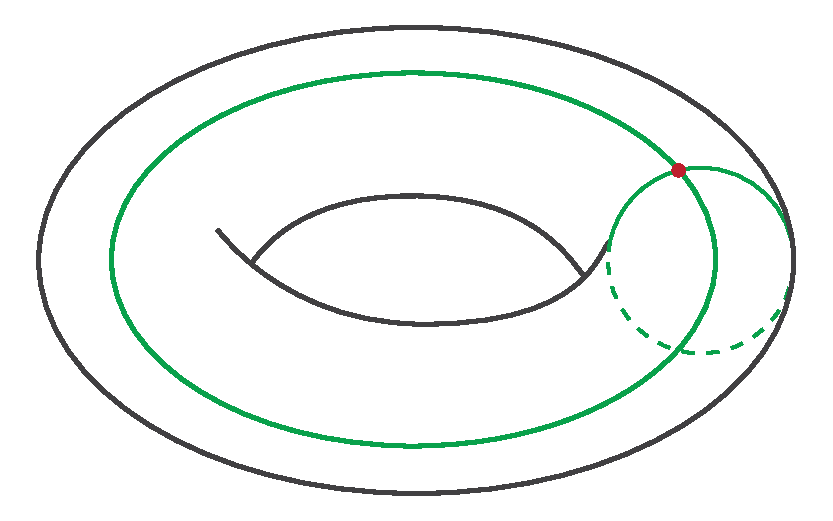
\includegraphics[trim=0cm 0cm 0cm 0cm, clip, scale=0.35]{images/torussubdivision.pdf}
		\end{center}
	\end{itemize}
\end{example}
\section{Caratteristica di Eulero}
\begin{definition}{}[Caratteristica di Eulero di una suddivisione]
	Data una suddivisione $\mathcal{S}$ di una superficie compatta $S$, essa avrà:
	\begin{itemize}
		\item $v$ vertici;
		\item $e$ lati;
		\item $f$ facce.
	\end{itemize}
La \textbf{caratteristica di Eulero}\index{caratteristica di Eulero} di $S$ rispetto alla suddivisione $\mathcal{S}$ è
\begin{equation*}
	\euler{S}{\mathcal{S}}=v-e+f\in\Z
\end{equation*}
\end{definition}
\begin{example}{pn}~{}
	\begin{itemize}
		\item Il \textit{tetraedro} ha 4 vertici, 6 lati e 4 facce, pertanto $S^2$ ha come caratteristica di Eulero $\euler{S}{\mathcal{S}_1}=4-6+4=2$.
		\item La suddivisione della sfera precedente, descritta da
		$\left(v,\ e,\ f\right)=\left(1,\ 1,\ 2\right)$, ha caratteristica di Eulero $\euler{S}{\mathcal{S}_1}=1-1+2=2$.
		\item Il toro ha una suddivisione $\left(v,\ e,\ f\right)=\left(1,\ 2,\ 1\right)$, con caratteristica di Eulero $\euler{S}{\mathcal{S}}=1-2+1=0$.
		\item Possiamo costruire una suddivisione alternativa del toro direttamente sul modello piano, nel modo seguente:
		\begin{center}
			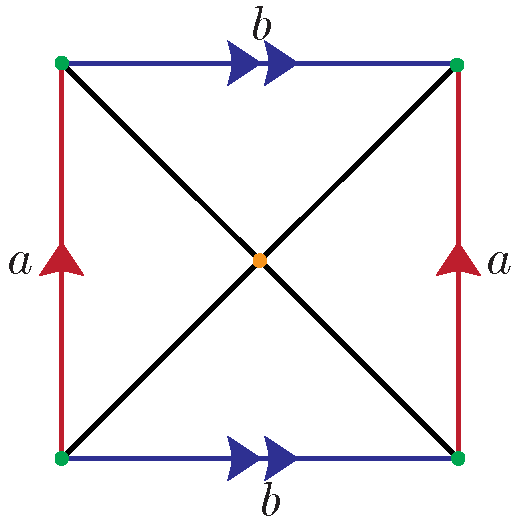
\includegraphics[trim=0cm 0cm 0cm 0cm, clip, scale=0.35]{images/torusmodelplane.pdf}
		\end{center}
	Abbiamo $\left(v,\ e,\ f\right)=\left(2,\ 6,\ 4\right)$ con caratteristica di Eulero $\euler{S}{\mathcal{S}}=2-5+4=0$.
	\end{itemize}
\end{example}
Notiamo che, in questi esempi, suddivisioni diverse di una stessa superficie hanno stessa caratteristica di Eulero. Questo \textit{non} è un caso: il seguente teorema, che non dimostreremo, ci garantisce ciò.
\begin{theorem}{q}[Caratteristica di Eulero indipendente dalla suddivisione]
Date due suddivisioni $\mathcal{S}_1$ e $\mathcal{S}_2$ della stessa superficie compatta $S$, si ha:
	\begin{equation*}
		\euler{S}{\mathcal{S}_1}=\euler{S}{\mathcal{S}_2}\qedhere
	\end{equation*}
\end{theorem}
\begin{definition}{}[Caratteristica di Eulero di una superficie]
	Sia $S$ una superficie compatta. La \textbf{caratteristica di Eulero} $\euler{S}{\ }\in \Z$ è la caratteristica di Eulero di una qualsiasi suddivisione di $S$.
\end{definition}
\begin{corollary}{n}[La caratteristica di Eulero è proprietà topologica]
\end{corollary}
\begin{proof}{n}
	Siano $S_1$ e $S_2$ due superfici compatte omeomorfe tra di loro e sia $\mathcal{S}_1$ una suddivisione di $S_1$. Usando l'omeomorfismo, costruiamo una suddivisione $\mathcal{S}_2$ di $S_2$ con lo stesso numero di vertici, lati e facce di $\mathcal{S}_1$. Allora:
	\begin{equation*}
		\euler{S_1}{\ }=\euler{S_1}{\mathcal{S}_1}=\euler{S_2}{\mathcal{S}_2}=\euler{S_2}{\ }\qedhere
	\end{equation*}
\end{proof}
\begin{example}{pn}~{}
	\begin{itemize}
		\item $\euler{S^2}{\ }=2$
		\item $\euler{T}{\ }=0$
	\end{itemize}
\end{example}
\subsection{Dimostrazione del teorema di classificazione: terza e ultima parte}
Forti di questo nuovo invariante per omeomorfismi, possiamo concludere la dimostrazione del teorema di classificazione delle superfici compatte. Innanzitutto, vediamo per bene che relazione c'è tra la caratteristica di Eulero e il modello piano di una superficie.
\begin{remark}{n}
	Sia $S$ una superficie compatta avente un modello piano con $2n$ lati identificati a coppie. Esso dà una suddivisione nativa di $S$ in cui:
	\begin{itemize}
		\item i \textit{vertici} $v$ sono le immagini in $S$ dei vertici del poligono e il loro numero è il numero di classi di equivalenza sui vertici del modello piano;
		\item i \textit{lati} $n$ sono le immagini in $S$ dei lati del poligono  e il loro numero è il numero di coppie di lati del modello piano;
		\item c'è solo \textit{una} faccia, data dall'immagine dell'interno del poligono.
	\end{itemize}
In altre parole:
\begin{equation*}
	\euler{S}{\ }=v-n+1
\end{equation*}
\end{remark}
\begin{proof}{n}~{}
	\begin{itemize}
		\item $P_n$ è espresso dalla parola $a_1a_1a_2a_2\ldots a_na_n$ e la suddivisione data dal modello piano ha un solo vertice, $n$ lati e una faccia. Allora
		\begin{equation*}
			\euler{P_n}{\ }=1-n+1=2-n\quad \forall n\geq 1.
		\end{equation*}
	In particolare,
	\begin{align*}
			\euler{P}{\ }&=1\\
			\euler{K}{\ }&=\euler{P_2}{\ }=0=\euler{T}{\ },
	\end{align*}
ma $T\ncong K$ in quanto $T$ è orientabile, mentre $K$ \textit{non} lo è. Notiamo che $\euler{P_n}{\ }\leq 1\ \forall n\geq 1$ e $\euler{P_n}{\ }= 2-n$ è una funzione iniettiva. Pertanto, se $n_1\neq n_2$, allora $\euler{P_{n_1}}{\ }\neq\euler{P_{n_2}}{\ }$ e, in quanto invariante per omeomorfismi, segue che $P_{n_1}\ncong P_{n_2}$. In altre parole, \textit{tutte} le superfici $P_n$ sono \textit{non} omeomorfe tra di loro.
\item $T_g$ è espresso dalla parola $a_1b_1a_1^{-1}b_1^{-1}\ldots a_nb_na_n^{-1}b_n^{-1}$ e la suddivisione data dal modello piano ha un solo vertice, $2g$ lati e una faccia. Allora
\begin{equation*}
	\euler{T_g}{\ }=1-2g+1=2-2g\quad \forall g\geq 1.
\end{equation*}
In particolare, se poniamo $T_0=S^2$ come caso ‘‘degenere'' di toro non bucato, $\euler{T_g}{\ }$ vale $\ \forall g\geq 0$. Dunque:
\begin{itemize}
	\item la caratteristica di Eulero delle superfici orientabili è sempre \textit{minore o uguale} a 2;
	\item $\euler{S}{\ }\leq 2$ per ogni superficie compatta.
\end{itemize}
Notiamo che $\euler{T_g}{\ }= 2-2g$ è una funzione iniettiva. Pertanto, se $g_1\neq g_2$, allora $\euler{T_{g_1}}{\ }\neq\euler{T_{g_2}}{\ }$ e, in quanto invariante per omeomorfismi, segue che $T_{g_1}\ncong T_{g_2}$. In altre parole, \textit{tutte} le superfici $T_g$ sono \textit{non} omeomorfe tra di loro.\qedhere
\end{itemize}
\end{proof}
\subsection{Somma connessa e caratteristica di Eulero}
\begin{lemma}{}[Caratteristica di Eulero della somma connessa]
	Siano $S_1,\ S_2$ due superfici compatte. Allora
	\begin{equation*}
		\euler{S_1\# S_2}{\ }=\euler{S_1}{\ }+\euler{S_2}{\ }-2.
	\end{equation*}
\end{lemma}
\begin{proof}{n}
	Scegliamo una triangolazione $\left(v_1,\ e_1,\ f_1\right)$ e $\left(v_2,\ e_2,\ f_2\right)$ per $S_1$ e $S_2$, rispettivamente. Per costruire $S_1\# S_2$ scegliamo un triangolo su $S_1$ e uno su $S_2$. Incolliamo le due superfici lungo i bordi di questi due triangoli. Otteniamo così una triangolazione per $S_1\# S_2$ con $\left(v_3,\ e_3,\ f_3\right)$ che soddisfa
	\begin{equation*}
			\begin{cases}
				v_3=v_1+v_2-3\\
				e_3=e_1+e_2-3\\
				f_3=f_1-1+f_2-1=f_1+f_2-2
			\end{cases}.
	\end{equation*}
	Allora
	\begin{equation*}
		\euler{S_1\# S_2}{\ }=v_3-e_3+f_3=v_1+v_2-\cancel{3}-\left(e_1+e_2-\cancel{3}\right)+f_1+f_2-2=\euler{S_1}{\ }+\euler{S_2}{\ }.\qedhere
	\end{equation*}
\end{proof}
\begin{remark}{n}
	Possiamo ora calcolare in un altro modo $\euler{P_n}{\ }$ e $\euler{T_g}{\ }$, per induzione:
	\begin{align*}
			\euler{P}{\ }&=1\\
			\euler{P_2}{\ }&=\euler{P\# P}{\ }=1+1-2=0\\
			\euler{P_n}{\ }&=\euler{P\# P_{n-1}}{\ }=\euler{P_n}{\ }+\euler{P_{n-1}}{\ }-2=1+2-\left(n-1\right)-2=2-n.
	\end{align*}
In modo analogo per $T_g$:
\begin{align*}
		\euler{T}{\ }&=0\\
		\euler{T_2}{\ }&=\euler{T\# T}{\ }=0+0-2=-2\\
		\euler{T_g}{\ }&=\euler{T\# T_{g-1}}{\ }=\euler{T_g}{\ }+\euler{T_{g-1}}{\ }-2=0+2-2\left(g-1\right)-2=2-2g.
\end{align*}
\end{remark}
\subsection{Impratichiamoci! Caratteristica di Eulero}
\begin{exercise}{}[Prova d'esame, Luglio 2018]
Sia $S$ la superficie compatta data dalla parola $abcdea^{-1}b^{-1}c^{-1}d^{-1}e^{-1}$. Determinare la classe di $S$ nella classificazione delle superfici compatte.
\end{exercise}
\begin{solution}{n}
	Tutte le coppie di lati sono del II tipo, pertanto $S$ è orientabile, cioè può essere $S^2$ o $T_g$ per un qualche $g\geq 1$, e la caratteristica di Eulero è del tipo $\euler{S}{\ }=2-2g$.\\
	$S$ ha un modello piano seguente con $10$ lati identificati a coppie, che dà origine ad una suddivisione di $S$ con 5 lati $a,\ b,\ c,\ d,\ e$, una faccia e $v$ vertici, con $v$ il numero di classi di equivalenza sui vertici del modello. Per calcolare $v$, disegniamo il modello piano e raggruppiamo i vertici:
	\begin{center}
		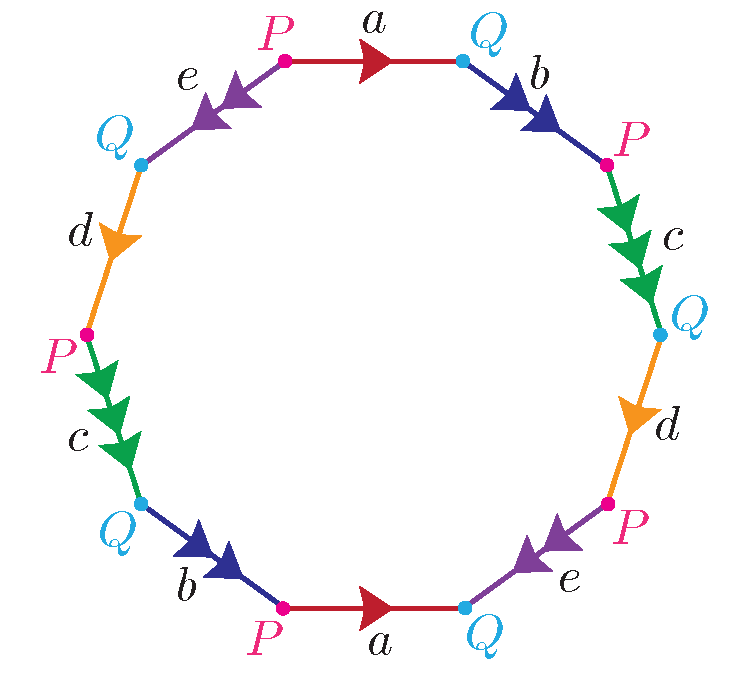
\includegraphics[trim=0cm 0cm 0cm 0cm, clip, scale=0.375]{images/modellopianoexercise.pdf}
	\end{center}
Su 10 vertici ho 2 classi di equivalenza, quindi $v=2$. Pertanto,
\begin{equation*}
	\euler{S}{\ }=v-5+1=2-4=-2=2-2g\implies 2g=4\implies g=2\implies S\cong T_2.
\end{equation*}
\end{solution}